% Import default values & document settings
% TODO replace TODOs with values
% Layout settings
\newcommand{\FIITdefaultFontSize}[0] {12pt}
\setcounter{secnumdepth}{3}
\setcounter{tocdepth}{3}

% Language settings
% \newcommand{\FIITlanguage}[0] {slovak}
\newcommand{\FIITlanguage}[0] {slovak,english}
\def\FIITlagEN{}

% Global texts
\newcommand{\FIITuniversity}[0] {Slovak University of Technology in Bratislava}
\newcommand{\FIITuniversitySK}[0] {Slovenská technická univerzita v Bratislave}
\newcommand{\FIITfaculty}[0] {Faculty of informatics and information technologies}
\newcommand{\FIITfacultySK}[0] {Fakulta informatiky a informačných technológií}
\newcommand{\FIITthesis}[0] {Progress report on DP1 solution}
\newcommand{\FIITthesisSK}[0] {Priebežná správa o riešení DP1}
\newcommand{\FIITtitle}[0] {Designing Zero-Knowledge Proof Solutions in Ethereum ecosystem}
\newcommand{\FIITtitleSK}[0] {Návrh riešení využívajúcich dôkazy s nulovým vedomím v Ethereum ekosystéme}
\newcommand{\FIITauthor}[0] {Lukáš Častven}
\newcommand{\FIITsupervisor}[0] {Ing. Kristián Košťál PhD.}
% \newcommand{\FIITevidenceNumber}[0] {TODO}
\newcommand{\FIITdate}[0] {May 2025}
\newcommand{\FIITdateSK}[0] {Máj 2025}
\newcommand{\FIITstudyProgram}[0] {Intelligent software systems}
\newcommand{\FIITstudyProgramSK}[0] {Inteligentné softvérové systémy}
\newcommand{\FIITstudyField}[0] {Computer Science}
% \newcommand{\FIITdegreeCourseSK}[0] {TODO}
\newcommand{\FIITinstitute}[0] {Institute of Computer Engineering and Applied Informatics}
\newcommand{\FIITinstituteSK}[0] {Ústav počítačového inžinierstva a aplikovanej informatiky}
\newcommand{\FIITsignPlace}[0] {In Bratislava, }
\newcommand{\FIITsignPlaceSK}[0] {V Bratislave, }
\newcommand{\FIITsignDate}[0] {31.5.2025}
% \newcommand{\FIITArchiveName}[0] {TODO}


% Setup document
\documentclass[\FIITdefaultFontSize,a4paper,twoside,openright,\FIITlanguage]{book}

% Load all necessary packages
\usepackage[final]{pdfpages}
\usepackage[utf8]{inputenc}
\usepackage[T1]{fontenc}
\usepackage[\FIITlanguage]{babel}
\usepackage[a4paper]{geometry}
\usepackage[
  left = \glqq,%
  right = \grqq,%
  leftsub = \glq,%
  rightsub = \grq%
]{dirtytalk}
\usepackage[parfill]{parskip}
\usepackage{enumitem}
\usepackage{calc}
\usepackage{graphicx}
\usepackage{float}
\usepackage{csquotes}
\usepackage{longtable}
\usepackage{setspace}
\usepackage{tabularx}
\usepackage{fancyhdr}
% Used to create the attachment doc \addto\captionsenglish{\renewcommand{\chaptername}{Attachment}}
\usepackage[backend=bibtex,sorting=none]{biblatex}
\usepackage{listing}
\usepackage{lscape}
\usepackage{afterpage}
\usepackage{hyperref}
\hypersetup{
    colorlinks=true,
    linkcolor=blue,
    filecolor=magenta,
    urlcolor=cyan,
    pdftitle={Overleaf Example},
    pdfpagemode=FullScreen,
    }
\usepackage{bera}
\usepackage{listings}
\usepackage{xcolor}
\usepackage{lipsum}
\usepackage{minted}
\usepackage{tikz}
\usepackage{tocloft}
\usepackage{amsfonts}
\usepackage{amsmath}
\usepackage{caption}
\usepackage{booktabs}

% Remove unnecessary gap between paragraph if large figure is inserted after them
\raggedbottom

% lscape.sty Produce landscape pages in a (mainly) portrait document.
\usepackage{lscape}

% Custom commands
\newcommand{\signaturespace}[2]{
  % #1 = width of the dotted line
  % #2 = legend
  \begingroup
  \renewcommand{\arraystretch}{0}
  \begin{tabular}[t]{cc}
    \hspace*{0pt}
    \cleaders\hbox{\kern.6pt.\kern.6pt}\hskip#1\relax
    \hspace*{0pt}
    \\[0.5cm]
    #2
  \end{tabular}
  \endgroup
}

\newcommand{\emptypage}{\newpage
  \thispagestyle{empty}
  \mbox{}
  \newpage}

% openright does not work :(
\let\tmp\oddsidemargin
\let\oddsidemargin\evensidemargin
\let\evensidemargin\tmp
\reversemarginpar


% Setup bibliography
\bibliography{bibliography}

% Page design
\pagestyle{fancy}
\lhead{\nouppercase{\leftmark}}
\chead{}
\rhead{}
\lfoot{}
\cfoot{\thepage}
\rfoot{}

\begin{document}

% Initialize document
% Layout
\setstretch{1.5}

% Bibliography
\ifx\FIITlagEN\undefined
  \defbibheading{references}[Zoznam použitej literatúry]{
    \chapter*{#1}
    \addcontentsline{toc}{chapter}{#1}
    \markboth{#1}{#1}
  }
  \defbibheading{referencessec}[Zoznam použitej literatúry]{
    \section*{#1}
    \markboth{#1}{#1}
  }
\else
  \defbibheading{references}[References]{
    \chapter*{#1}
    \addcontentsline{toc}{chapter}{#1}
    \markboth{#1}{#1}
  }
  \defbibheading{referencessec}[References]{
    \section*{#1}
    \markboth{#1}{#1}
  }
\fi

% Syntax highlighting
\setminted[]{linenos,tabsize=2,breaklines}
\colorlet{punct}{red!60!black}
\definecolor{background}{HTML}{EEEEEE}
\definecolor{delim}{RGB}{20,105,176}
\colorlet{numb}{magenta!60!black}

% Text highlighting
\makeatletter
\newenvironment{btHighlight}[1][]
{\begingroup\tikzset{bt@Highlight@par/.style={#1}}\begin{lrbox}{\@tempboxa}}
    {\end{lrbox}\bt@HL@box[bt@Highlight@par]{\@tempboxa}\endgroup}

\newcommand\btHL[1][]{%
  \begin{btHighlight}[#1]\bgroup\aftergroup\bt@HL@endenv%
    }
    \def\bt@HL@endenv{%
  \end{btHighlight}%   
  \egroup
}
\newcommand{\bt@HL@box}[2][]{%
  \tikz[#1]{%
    \pgfpathrectangle{\pgfpoint{1pt}{0pt}}{\pgfpoint{\wd #2}{\ht #2}}%
    \pgfusepath{use as bounding box}%
    \node[anchor=base west, fill=black!10,outer sep=0pt,inner xsep=1pt, inner ysep=-2pt, rounded corners=3pt, minimum height=\ht\strutbox+1pt,#1]{\raisebox{1pt}{\strut}\strut\usebox{#2}};
  }%
}
\makeatother

\newcommand{\createFigure}[2]{
    \begin{figure}[h]
        \centering
        \includegraphics[width=\textwidth]{#1}
        \caption{#2}
        \vspace{0.5cm}
    \end{figure}
}

\newenvironment{tikzFigure}{
	\begin{figure}[htbp]
		\vspace{0.5cm}
        \centering
	}
	{
		\vspace{0.5cm}
	\end{figure}
}


% Cover & title page
% Cover page
\begin{center}
    \thispagestyle{empty}
    \ifx\FIITlagEN\undefined
    {\Large \FIITuniversitySK}
    \else
    {\Large \FIITuniversity}
    \fi
\par\end{center}{\Large \par}

\begin{center}
    \ifx\FIITlagEN\undefined
    {\Large \FIITfacultySK}
    \else
    {\Large \FIITfaculty}
    \fi
\par\end{center}{\Large \par}

\smallskip{}

\begin{center}
    \ifx\FIITlagEN\undefined
    Evidenčné číslo: \FIITevidenceNumber
    \else
    Reg. No.: \FIITevidenceNumber
    \fi
\par\end{center}
\vfill{}

\begin{center}
    \textbf{\Large \FIITauthor}
\par\end{center}{\Large \par}

\medskip{}


\begin{center}
    \ifx\FIITlagEN\undefined
    \textbf{\LARGE \FIITtitleSK}
    \else
    \textbf{\LARGE \FIITtitle}
    \fi
\par\end{center}{\huge \par}

\medskip{}


\begin{center}

    \ifx\FIITlagEN\undefined
    {\Large \FIITthesisSK}
    \else
    {\Large \FIITthesis}
    \fi
\par\end{center}{\Large \par}

\vfill{}


\ifx\FIITlagEN\undefined
Vedúci záverečnej práce: \FIITsupervisor
\else
Thesis supervisor: \FIITsupervisor
\fi

\medskip{}

\ifx\FIITlagEN\undefined
\FIITdateSK
\else
\FIITdate
\fi

\pagenumbering{roman}
\emptypage





% Thesis title page
\begin{center}
    \thispagestyle{empty}
    \ifx\FIITlagEN\undefined
    {\Large \FIITuniversitySK}
    \else
    {\Large \FIITuniversity}
    \fi
\par\end{center}{\Large \par}

\begin{center}
    \ifx\FIITlagEN\undefined
    {\Large \FIITfacultySK}
    \else
    {\Large \FIITfaculty}
    \fi
\par\end{center}{\Large \par}

\smallskip{}

\begin{center}
    \ifx\FIITlagEN\undefined
    Evidenčné číslo: \FIITevidenceNumber
    \else
    Reg. No.: \FIITevidenceNumber
    \fi
\par\end{center}
\vfill{}

\begin{center}
    \textbf{\Large \FIITauthor}
\par\end{center}{\Large \par}

\medskip{}


\begin{center}
    \ifx\FIITlagEN\undefined
    \textbf{\LARGE \FIITtitleSK}
    \else
    \textbf{\LARGE \FIITtitle}
    \fi
\par\end{center}{\huge \par}

\medskip{}


\begin{center}

    \ifx\FIITlagEN\undefined
    {\Large \FIITthesisSK}
    \else
    {\Large \FIITthesis}
    \fi
\par\end{center}{\Large \par}

\vfill{}


\ifx\FIITlagEN\undefined
Študijný program: \FIITstudyProgramSK

Študijný odbor: \FIITdegreeCourseSK

Školiace pracovisko: \FIITinstituteSK

Vedúci záverečnej práce: \FIITsupervisor
\else
Study programme: \FIITstudyProgram

Study field: \FIITstudyField

Training workplace: \FIITinstitute

Thesis supervisor: \FIITsupervisor
\fi

\medskip{}

\ifx\FIITlagEN\undefined
\FIITdateSK
\else
\FIITdate
\fi

\emptypage


% TODO Thesis assignment
% \newpage
% \thispagestyle{empty}
% \begin{center}
%     
\includegraphics[width=\textwidth]{assets/assignment.pdf}
% \end{center}
% \newpage
% \emptypage


% TODO Declaration of honor
% \thispagestyle{empty}


\section*{Čestné prehlásenie}

\vspace*{\fill}

Čestne vyhlasujem, že som túto prácu vypracoval(a) samostatne, na základe konzultácií
a s použitím uvedenej literatúry.

\FIITsignPlaceSK \FIITsignDate
\hspace*{\fill} \signaturespace{5cm}{\FIITauthor}


% TODO Annotation
% % Annotation in Slovak
\thispagestyle{empty}

\vspace*{\fill}

\section*{Anotácia}

\begin{minipage}[t]{1\columnwidth}
    \FIITuniversitySK

    \FIITfacultySK

    Študijný program: \FIITstudyProgramSK\\

    Autor: \FIITauthor

    \FIITthesisSK: \FIITtitleSK

    Vedúci bakalárskej práce: \FIITsupervisor

    \FIITdateSK
\end{minipage}

\bigskip{}

Táto práca skúma návrh a potenciálnu implementáciu riešení využívajúcich
dôkazy s nulovým vedomím (ZKP) v rámci ekosystému Ethereum, s cieľom riešiť
problémy škálovateľnosti a dosiahnuť post-kvantovú bezpečnosť. Dôkazy s
nulovým vedomím sú kryptografické metódy, ktoré umožňujú overenie integrity
výpočtov bez odhalenia citlivých dát, čo ich robí mimoriadne vhodnými pre
zlepšenie súkromia a efektivity v blockchainových systémoch. Ústredným
zameraním tejto práce je prieskum Zero-Knowledge Virtual Machine (ZkVM)
prispôsobenej pre inštrukčnú sadu RISC-V, s využitím princípov kryptografie
založenej na mriežkach. Kľúčovou aplikáciou takéhoto ZkVM by bolo dokázateľne
spávne vykonanie Ethereum blokov cez ZkEVM.

Výskum zahŕňa analýzu architektúry Ethereum, konceptu "snarkifikácie" pre
konsenzuálnu aj exekučnú vrstvu, evolúciu a prirodzené výzvy ZkEVM (vrátane
rekurzívnych dôkazov a skladacích schém), a preskúmanie kryptografických
primitív založených na mriežkach, ako sú Ajtaiho záväzky, spolu so súčasnými
systémami LaBRADOR, Greyhound a LatticeFold/LatticeFold+.

Cieľom tejto diplomovej práce je prispieť do odboru zhodnotením potenciálnej
výkonnosti ZKP systémov postavených na kryptografii založenej na mriežkach pre
úlohu dokazovania správneho vykonania Ethereum blokov. Práca sa ďalej snaží
porovnať tieto nové riešenia s etablovanými klasickými ZKP prístupmi, pričom
zachováva post-kvantovú odolnosť.


\newpage{}\thispagestyle{empty}\medskip{}

% Annotation in English
\thispagestyle{empty}

\vspace*{\fill}

\section*{Annotation}

\begin{minipage}[t]{1\columnwidth}
    \FIITuniversity

    \FIITfaculty

    Degree Course: \FIITstudyProgram\\

    Author: \FIITauthor

    \FIITthesis: \FIITtitle

    Supervisor: \FIITsupervisor

    \FIITdate
\end{minipage}

\bigskip{}

This thesis explores the design and potential implementation of
solutions utilizing Zero-Knowledge Proofs (ZKPs) within the Ethereum
ecosystem, aiming to address scalability challenges and achieve post-quantum
security. ZKPs are cryptographic methods that allow the verification of
computational integrity without revealing sensitive data, making them
suitable for improving privacy and efficiency in blockchain systems. The
central focus of this work is the exploration of a Zero-Knowledge Virtual
Machine (ZkVM) for the RISC-V instruction set, leveraging lattice-based
cryptography. A key application of such a ZkVM would be to enable creating
proofs of correct execution of EVM.

The research includes an analysis of Ethereum's architecture, the concept of
"snarkification" for both consensus and execution layers, the evolution and
challenges of ZkEVMs (recursive proofs and folding schemes), and an
examination of lattice-based cryptographic primitives, such as Ajtai
commitments, along with contemporary systems like LaBRADOR, Greyhound, and
LatticeFold/LatticeFold+.

This engineer's thesis aims to contribute to the field by evaluating the
potential performance of ZKP systems built on lattice-based cryptography for
the task of proving the correct execution of Ethereum blocks. The work further
seeks to compare these emerging solutions with established classical ZKP
approaches, while maintaining post-quantum resistance.

\newpage{}\thispagestyle{empty}

\emptypage


% Table of contents
\ifx\FIITlagEN\undefined
    \renewcommand{\contentsname}{Obsah}
\else
    \renewcommand{\contentsname}{Table of contents}
\fi
\tableofcontents{}

% List of figures
\listoffigures

% List of abbreviations
\thispagestyle{plain}

\ifx\FIITlagEN\undefined
    \section*{\Huge Zoznam použitých skratiek}
    \markboth{Zoznam použitých skratiek}{Zoznam použitých skratiek}
\else
    \section*{\Huge List of abbreviations used}
    \markboth{List of abbreviations used}{List of abbreviations used}
\fi
\vskip 1cm

\begin{tabular}{ >{\bfseries}m{2cm} m{10cm} }
	ERC & Ethereum Request for Comments \\
	EVM & Ethereum Virtual Machine 	\\
	SNARK & Succinct Non-interactive Argument of Knowledge \\
	R1CS & Rank-1 Constraint System \\
	ZK  & Zero Knowledge           	\\
	ZKP & Zero Knowledge Proof
\end{tabular}

\emptypage


% Enable page numbering
\pagenumbering{arabic}

% Begin references segment
\begin{refsegment}

% the analysis structure:
	% TODO turn these chapters into sections with an analysis chapter as parent
%	1. ethereum
%		a. consensus
%		b. execution layer
%	2. snarkification
%		a. ZKPs
%		b. snarkification benefits, why and how
%		c. beam chain - snarkification of consensus
%		d. enshrined zkEVM - snarkification of execution
% 	3. execution layer snarkification => zkEVM, what it is
%		a. RISC-V zkVMs with EVMs binaries compiled to RISC-V
%		b. nowadays -> recursion and folding
%		c. comparison of different zkVMs/zkEVMs (https://ethproofs.org/)
%	4. Proposed lattice based ZK system
%		a. LatticeFold
%		b. LABRADOR/Greyhound for final check
% 	5. Goal: prove ethereum blocks with lattices. Simple question, are lattice
%		based ZK systems viable to prove ETH blocks? And on what hardware?

    \section{Ethereum}\label{sub:ethereum}

Ethereum is a decentralized, open-source blockchain with smart contract
functionality \cite{ethereumEthereumWhitepaper}. Conceptualized by Vitalik
Buterin in 2013/2014, it went live in 2015, aiming to build a platform for
decentralized applications that adds Turing complete execution environment
to blockchain \cite{ethereumWhitePaperPdf}. Ethereum enables developers to
create and deploy decentralized applications and crypto assets.
The Ethereum network is comprised of two layers, two peer-to-peer networks,
consensus layer and execution layer.

\subsection{Consensus}\label{subsec:ethereum_consensus}
% very good explainer https://ethos.dev/beacon-chain

Consensus on Ethereum is achieved with proof-of-stake (PoS) consensus mechanism
called Gasper \cite{VitalikGasper}. PoS system relies on crypto-economic incentives,
rewarding honest stakers (people who put economic capital in the network)
and penalizing malicious ones.

Stakers, or also called validators, propose new blocks. Validator is selected for
a block proposal pseudo-randomly from the pool in each slot. A slot is some
time amount (as of writing of this work it is 12 seconds on Ethereum mainnet),
in which the pseudo-randomly chosen validator can propose new block. The software
creating the new block is called consensus client. Proposer's consensus client
requests a bundle of transactions from the execution layer \ref{subsec:ethereum_execution},
wraps them into a block and gossips (sends) the new block to other participants
over the consensus p2p network. The rest of the validator pool can in 32 slot
(or one epoch) attest to that new block's validity. In order for a block to be
finalized, it must be attested by a super-majority, which is 66\% of the total
balance of all validators. \cite{ethereumConsensusMechanisms}.

\subsection{Execution}\label{subsec:ethereum_execution}

Software operating on the execution layer is called execution client. Nodes on
execution layer hold the latest state and database of all Ethereum data. These
clients gossip incoming transactions over the execution layer p2p network, and
each stores them in a local mempool. Once they are put inside a block, each
transaction is executed in Ethereum-Virtual-Machine (EVM). EVM is a stack based
virtual machine operating 256 bit words which executes smart contract code.
Ethereum is a decentralized state machine, with rules defined by the EVM.
EVM can be thought of as a function. Given a valid state and valid set of
transactions\footnote{validity of transactions, and thus transitively validity
of state, is guaranteed by the consensus layer \ref{subsec:ethereum_consensus}},
outputs next valid state:

\[
	F(S_n, T) = S_{n+1} \label{eq:state_transition}
\]

Thus, Ethereum's state transition function is described by the EVM. This function
must be executed by each execution node for each new block in order to keep up
with the current chain state. \cite{ethereumEthereumVirtual}



    \section{Snarkification of Ethereum}\label{sec:snarkification}

As discussed in sections on consensus (\ref{subsec:ethereum_consensus}) and
execution layer (\ref{subsec:ethereum_execution}), nodes on each layer must expend
compute resources to validate the consensus data of new blocks or re-execute all
transactions within them to verify and maintain the blockchain's state.
These computational demands limit the scalability of the entire network.

Ethereum's decentralized node network includes not only participants with
capable servers, but also hobbyists, who use home internet connections and
less powerful machines. Naively attempting to scale the network, for instance,
by decreasing slot time, or increasing block size may raise bandwidth and node
requirements, thereby ousting less capable nodes and thus hindering Ethereum's
decentralization.

Snarkification refers to the process of integrating specific type of Zero
Knowledge Proofs (ZKPs) called SNARK (Succinct Non-interactive Argument of
Knowledge) in order to offload a computation to one entity (one node, or a
cluster that is a small subset of the whole network), which performs the
computation and generates a proof of its validity. This proof can then be
verified by the rest of the network at fractional compute cost.

\subsection{Zero Knowledge Proofs}

Zero-Knowledge Proofs are cryptographic primitives that allow a prover
to convince a verifier of a statement's truth without revealing any
information beyond the statement's validity itself. The statement typically
concerns membership in an NP language/relation \cite{GoldreichNPProofs}.
The membership statements are usually named ZK circuits.
Traditionally, ZKPs are interactive protocols where a prover, knows a
private witness for a statement (e.g., a solution to a problem), aims to
convince a verifier of this knowledge. Through a series of back-and-forth
interactions, the verifier becomes convinced of the prover's claim (if true)
without learning the witness itself.

Interactive proofs where the verifier's messages consist only of random
challenges are known as public-coin protocols. The Fiat-Shamir heuristic \cite{FiatShamir}
can transform such public-coin interactive proofs into non-interactive
proofs by replacing the verifier's random challenges with challenges derived
from a cryptographic hash function applied to the protocol's transcript. This
non-interactivity allows a single generated proof to be validated by any
number of verifiers.

A SNARK is a specific type of ZKP. The 'Succinct' aspect implies that proof
sizes are very small (e.g., polylogarithmic in the size of the witness or
statement) and verification is faster than re-executing the original
computation, often polylogarithmic in the computation's complexity \cite{BCCT11}.

\subsection{Snarkifying consensus}

The 'Beam Chain' is a research initiative, introduced by Justin Drake at Devcon
2024 \cite{JustinDrakeBeamchain}, aimed at redesigning and improving
Ethereum's consensus mechanism. A key aspect of this proposal involves
leveraging SNARKs to make consensus layer state transitions provable, in near
real-time. Instead of each validator independently re-validating all
components of a new consensus state, they would verify a single, compact
SNARK. Based on this proof's validity, they would accept or
reject the proposed state update.\footnote{The entity proposing the state
update, such as a block proposer, would be responsible for generating and
submitting this proof.}

\subsection{Snarkifying execution}\label{subsec:snarkifying_execution}

Ethereum's execution state transitions are dictated by the rules of the
EVM. To reduce the computational burden of verifying execution using ZKPs, the
EVM's execution logic needs to be provable with a ZKPs, creating a ZkEVM. This
would change the state transition function (\ref{eq:state_transition}) to:

\[
	F(S_n, T) = (S_{n+1}, \pi)
\]

Where $\pi$ is the proof of the state transition's validity. Therefore,
verifying a block's execution state transition would involve verifying this
single proof, rather than re-executing all transactions within the block.
Furthermore, an increase in block size would have a little to no impact on
verification times for nodes, as proof verification complexity typically grows
much slower than the computation being proven. This could allow for larger
block sizes without risking the exclusion of nodes with modest computational
capabilities due to their weaker computational capabilities, thereby
supporting scalability.

Another approach is to 'enshrine' a ZkEVM directly into the Ethereum protocol (L1).
This offers similar benefits in terms of L1 state transition verification, as
the native EVM could delegate execution proving to this enshrined ZkEVM. In
addition, an enshrined ZkEVM could support and simplify the creation of what
are sometimes termed 'native rollups' \cite{NativeRollups}. These would be
Layer 2 solutions that could leverage the L1's enshrined ZkEVM for verifying
their own state transitions, which are themselves batches of EVM-compatible
transactions. The correctness of these L2 transaction batches would thus be
directly enforced by the L1 execution layer through ZK proof verification.
This could lead to faster, settlement for these L2s on L1, which in turn could
simplify composability between L1 and these native L2s, as well as among
different native L2s.



    % \chapter{Introduction}

Ethereum, a decentralized blockchain platform launched in 2015, provides a
Turing-complete execution environment for smart contracts and decentralized
applications. Its modular architecture comprises a proof-of-stake consensus
layer (Gasper) and an execution layer governed by the Ethereum Virtual Machine
(EVM). A primary challenge for Ethereum is scalability, as the need for all
nodes to validate and re-execute every transaction limits throughput and can
centralize the network by increasing resource demands.

"Snarkification," the integration of Zero-Knowledge Proofs (ZKPs) like SNARKs,
offers a path to mitigate these scalability issues. Initiatives such as the
'Beam Chain' aim to snarkify consensus, allowing validators to verify compact
proofs instead of entire state components. Similarly, Zero-Knowledge Ethereum
Virtual Machines (ZkEVMs) seek to make EVM execution provable, enabling nodes
to verify block execution via a single proof. Enshrining a ZkEVM into
Ethereum's Layer 1 could further enhance scalability and simplify the creation
of native rollups.

Zero-Knowledge proofs allow proving a statement's truth without revealing
underlying information. The statement are usually a membership in NP language,
thus an entire computations can be proven with this primitives, for example
like computations done by the EVM, turning it into a ZkEVM. However,
developing ZkEVMs is challenging due to the EVM's original design: complex
opcodes, large word sizes requiring range proofs, its stack-based nature, and
ZK-unfriendly storage mechanisms. Early solutions utilized recursive proofs to
aggregate computation steps, leading to the first generation of Layer 2
ZkEVMs. Folding schemes further optimized this by compressing instances. The
current trend involves Zero-Knowledge Virtual Machines (ZkVMs), especially
those based on the simpler, register-based RISC-V ISA, which is more amenable
to ZK proof generation.

While many ZKP systems rely on assumptions vulnerable to quantum attacks,
lattice-based cryptography provides a foundation for post-quantum secure ZK
solutions, with security often based on hard problems like SVP or SIS.

This thesis investigates the design and implementation of a RISC-V ZkVM using
lattice-based cryptography. A key application is proving Ethereum block
execution, contributing to the network's scalability and post-quantum
security. This work explores the practical construction of such a system and
aims to assess whether lattice-based cryptography can offer performance
comparable to classical ZKP methods while ensuring quantum resistance.

\section*{Document Structure}

This progress report on the DP1 solution details the initial analytical work
in Analysis \ref{chap:analysis}. This chapter begins with an overview of
Ethereum \ref{sec:ethereum}, covering its consensus and execution mechanisms.
It then explores the concept of Snarkification of Ethereum \ref{sec:snarkification},
discussing Zero-Knowledge Proofs and their application to both the consensus
layer via the Beam Chain initiative and the execution layer through enshrined
ZkEVMs. Following this, the report analyzes ZkEVMs \ref{sec:zkevm},
examining the challenges of proving EVM execution, the evolution of solutions
from recursive proofs and folding schemes to modern ZkVMs. Finally, the
analysis introduces Lattice-based cryptography \ref{sec:lattices}, outlining
Ajtai commitments and the potential of lattices for post-quantum
zero-knowledge systems, including recent developments like LaBRADOR,
Greyhound, and LatticeFold/LatticeFold+.

    %
    % \chapter{Analysis}\label{analysis}

This chapter, analyzes shift towards smaller prime fields in
ZKP systems to enhance efficiency and data density.
Section~\ref{analysis:smaller-prime-fields} discusses the shift from large
fields to smaller ones, highlighting protocols like Plonky2, STWO, and Plonky3
that leverage smaller primes for improved performance. Section~\ref{analysis:binary-fields}
delves into the use of binary field ($\mathbb{F}_2$), exploring their
computational advantages and the protocol proposed by Diamond and Posen
\cite{Binius} that utilizes towers of binary fields. Aim of this chapter is to
understand the potential benefits and challenges of adopting smaller and
binary fields in ZKP proving systems.

\section{Smaller prime fields}\label{analysis:smaller-prime-fields}

Today's ZK proving systems work over a large primary fields of bit size $2^{256}$.
However, the majority of programs use small numbers. Indices of arrays,
variables with 64 bit size, or values representing single bit (true or false)
use only a fraction of the whole $2^{256}$ field, thus creating an inefficiency
and decreasing the information density.

Current trend and research directions tend towards using smaller prime fields.
SNARKs over a elliptic curves become insecure when smaller prime fields are used.
On the other hand, STARKs \cite{SassonSTARKs} use different approach based on hashing.
This make it possible to reduce the size of the field. Plonky2 \cite{Plonky2}
started this by performing calculation over a $2^{64}$, which improved the proof
generation performance. Starkware's stwo \cite{CircleStarks} and Plonky3 \cite{Plonky3}
shrink the underlying field size further with usage of Mersenne prime $2^{31} - 1$.

\section{Binary field}\label{analysis:binary-fields}

This tendency to shrink underlying field has a logical conclusion, a field over
the smallest prime, 2. This field has a beautiful properties when computation is
done in it. Addition is a bitwise XOR without the need to carry. Squaring elements
is less expensive than multiplying two elements, due to the fact that in this
field $(x + y)^2 = x^2 + y^2$ (this property can be referred to as "Freshman's
dream \cite{FreshmansDream}).

Diamond and Posen in \cite{Binius} propose a protocol constructed from binary
field and binary tower of fields ($F_2 \subset F_{2^2} \subset F_{2^3}
\ldots$). The binary field can be extended as many 
times as needed \cite{Wiedemann86}. By using the binary field, data of size
$n$ will be encoded in $n$ bits, and hence creating a dense encoding.

Multilinear polynomial is committed with a Merkle tree. In order to
encode a polynomial representing large set of values, they need to be
accessible as evaluations of the polynomial and used field must contain such
values. So, the values (the trace of the computation) are encoded as points on
hypercube $P(x_0, x_1, \ldots, x_k)$. Then to prove evaluations at random
points, the data is interpreted as a square, extended with Reed-Solomon
encoding. This gives the data redundancy for random Merkle tree queries, so
that the evaluation is secure. And thanks to the binary field, the integers
produced by extending with Reed-Solomon do not blow up.

The proposed protocol has a $\mathcal{O}(\sqrt{N})$ verification time and
for a proof of $2^{32}$ bits around 11MB is needed.


    %
    % \chapter{Related work}\label{chapter:related}

With the growth of cryptocurrencies, ZKPs have gained a substantial popularity
not only in academic circles, but also in the startup and venture capital
ones. Many researchers are studying this field and it is not considered 
as a cryptography for nerds anymore. 

On the other hand, there are not many contributions to the stealth address
ecosystem. This field gets some traction, for example, work done by
Fan, Jia and Wang, Zhen and Luo, Yili and Bai, Jian and Li, Yarong and Hao, Yao
\cite{FanJiaWang2019} introduce a stealth address scheme designed to
enhance user privacy in blockchain transactions. The scheme aims to address
the limitations of existing solutions, such as the need for users to manage
multiple key pairs or engage in additional private communication before each
transaction. In their approach, a user only needs to maintain a single key
pair for initial certification, simplifying key management and reducing
storage costs. The sender creates a one-time transaction address and attaches
it to the transaction, while the receiver utilizes their private key to verify
the transaction directly from the blockchain, eliminating the need for a
separate private channel. The scheme also offers flexibility for regulation,
allowing transactions to be either fully or partially regulated based on
security requirements.

Or, Wang \cite{Wang2023} introduced the concept of Fast Stealth Addresses (FSAs)
to improve the search efficiency of stealth address schemes in blockchain transactions.
Their approach aims to overcome the linear search time required in existing schemes
by allowing constant recognition time to determine if a block contains a recipient's
transactions and logarithmic search time to locate the specific transactions.
The authors provide a generic construction of the FSA scheme under subgroup membership
assumptions related to factoring and instantiate concrete schemes based on specific
number-theoretic assumptions. They also formalize the security model of an FSA
scheme and provide provable security analysis.

There are two protocols on Ethereum that implement stealth addresses.
First one is called Nocturne \cite{nocturne}. The protocol is a mix of
elliptic curve cryptography and ZKPs with few intermediate smart contracts.
In this protocol you lock your funds in the Nocturne ecosystem, in which
new stealth addresses are created with Elliptic curve stealth addresses scheme,
and you access your funds by submitting ZKPs. However according to their
\href{https://twitter.com/nocturne_xyz/status/1749510390906511693}{Twitter post}
they are discontinuing their protocol.

The second one is called Umbra \cite{umbra}. Umbra is a protocol on Ethereum
that implements stealth addresses using elliptic curve cryptography. In this
protocol, the recipient a private keys. The sender generates a random number,
encrypts it using the recipient's public key, and then
computes the stealth address from the recipient's public key and the random
number. The encrypted random number, ephemeral public key, and stealth address
are then published. The recipient can scan these announcements, decrypt the
random number using their private key, and check if the derived stealth
address matches the one in the announcement. If it does, they can then use
their spending key to access the funds.

Kovács and Seres \cite{Kovacs2023} conducted an analysis of Umbra's recipient
anonymity guarantees on Ethereum and its layer-2 solutions. They identified four
heuristics based on user behavior that could compromise the anonymity and
linkability of Umbra transactions. These heuristics exploit patterns such as
the reuse of registrant addresses, the overlap of sender and receiver
addresses, the collection of multiple payments to a single address, and unique
transaction fees. The study found that a significant portion of Umbra
transactions could be deanonymized using these heuristics, raising concerns
about the protocol's privacy in practice. The authors suggest countermeasures
such as avoiding address reuse and using different addresses for different
on-chain activities to mitigate these risks.


    %
    % \chapter{Solution Design}\label{chapter:solution}

The core problem this thesis addresses is the inherent lack of privacy in
blockchain transactions. While blockchains like Ethereum offer transparency
and security, the public nature of transactions exposes user identities and
financial activities, raising significant privacy concerns. This work
introduces a novel solution to this problem by ZKPs to create a stealth
address scheme.

The key novelty and scientific contribution of this thesis lie in the design
and implementation of a proof-of-concept stealth address scheme that utilizes
ZKPs. This scheme allows users to receive funds without publicly revealing
their identities, enhancing privacy in blockchain transactions. The proposed
solution enables the creation of stealth addresses derived from the
recipient's public data, ensuring that only the recipient can control and
access the funds sent to these addresses. The use of ZKPs allows the recipient
to prove ownership of the stealth address without disclosing any private
information, thus preserving anonymity.

Furthermore, this thesis contributes to the field by demonstrating the
practical application of ZKPs in addressing real-world privacy challenges in
blockchain technology. By presenting a conceptual implementation of the
stealth address scheme, this work showcases the potential of ZKPs to enhance
privacy and security in blockchain applications.

The Solution Design section outlines the design of a stealth address
scheme utilizing ZKPs. The scenario which is being solved involves Alice
(sender), who wishes to send funds to Bob (recipient)
discreetly, ensuring no one else can identify Bob as the recipient, and that
only Bob can control the funds sent. This part of the
thesis details the application of ZKPs to achieve this privacy,
allowing Alice to complete the transaction without compromising Bob's identity.

\section{Requirements}

The solution enables a proof of concept stealth wallet. This will not be a
full featured wallet, only one satisfying these requirements:

\subsection*{Functional requirements}
\begin{itemize}
    \item \textbf{Meta Stealth Address Retrieval:} The solution must enable senders
        to query and retrieve meta stealth addresses from the registry.
    \item \textbf{Ephemeral Key Exchange:} The solution needs a mechanism for senders
        to submit ephemeral keys and owners to query them.
    \item \textbf{Stealth Wallet Deployment:} Senders must be able to deploy
        stealth wallet smart contracts, specifying the code and depositing funds.
    \item \textbf{Zero-Knowledge Proof Generation:} The solution must provide a way
        for owners to generate ZKPs that demonstrate ownership.
    \item \textbf{Zero-Knowledge Proof Verification:} Smart contracts must be able
        to verify the ZKPs submitted by owners.
    \item \textbf{Stealth Wallet Withdrawal:} Upon successful ZKP
        verification, the smart contract must execute a withdrawal, transferring
        the entire stealth wallet balance to the owner's designated address.
\end{itemize}

\subsection*{Non-functional requirements}
\begin{itemize}
    \item \textbf{Security:} The solution must prioritize the protection of private keys.
    \item \textbf{Privacy:} Stealth addresses and the link between owners and
        their stealth wallets should be obscured to preserve on-chain privacy.
    \item \textbf{Compatibility:} The solution should be compatible with
        relevant Ethereum testnet environment, not only a local
        development environment.
\end{itemize}


\section{High Level Overview}

The main idea behind the solution is a fact that both
receiver and sender generate a private random value. These two values can then
be used to prove to a stealth address that whoever owns these values
is the owner of the stealth address, and can control it.

Bob, as a receiver, only publishes the hash of his random value. Alice then
generates her own random value and hashes it with Bob's hash to create a
code which will be submitted to the stealth address contract. After that, she
encrypts her random value, and address of the new stealth address
contract with Bob's public key. This is called ephemeral key, and it is published
to a public registry. Bob then scans the registry, decrypts the ephemeral key and
saves Alice's secret value and the address of the contract with funds from Alice.

When Bob wants to use the funds, he submits a proof to the stealth address
contract. This proof proves that Bob knows Alice's random value and his own
random value, such that the combination of hash of Bob's secret value and
Alice's secret value is equal to the code submitted by Alice into the stealth
address contract. Also, to prevent others from copying the proof when Bob
sends it in a transaction, and gaining control over the stealth address with a higher fee
transaction, the proof must verify the sender of the transaction. In the
proof, there must be a check that the address with which Bob wants to interact
with the stealth wallet is the one sending the transaction. Without this check
a malicious actor could copy the proof and send a transaction with higher fee,
which would give him access to the address sooner, because it would be placed
higher in the block. Since only Bob knows both secret values and an address
from which he will be sending transaction, only he can create a valid
proof and thus interact with the address.

\begin{figure}[h]
    \centering
    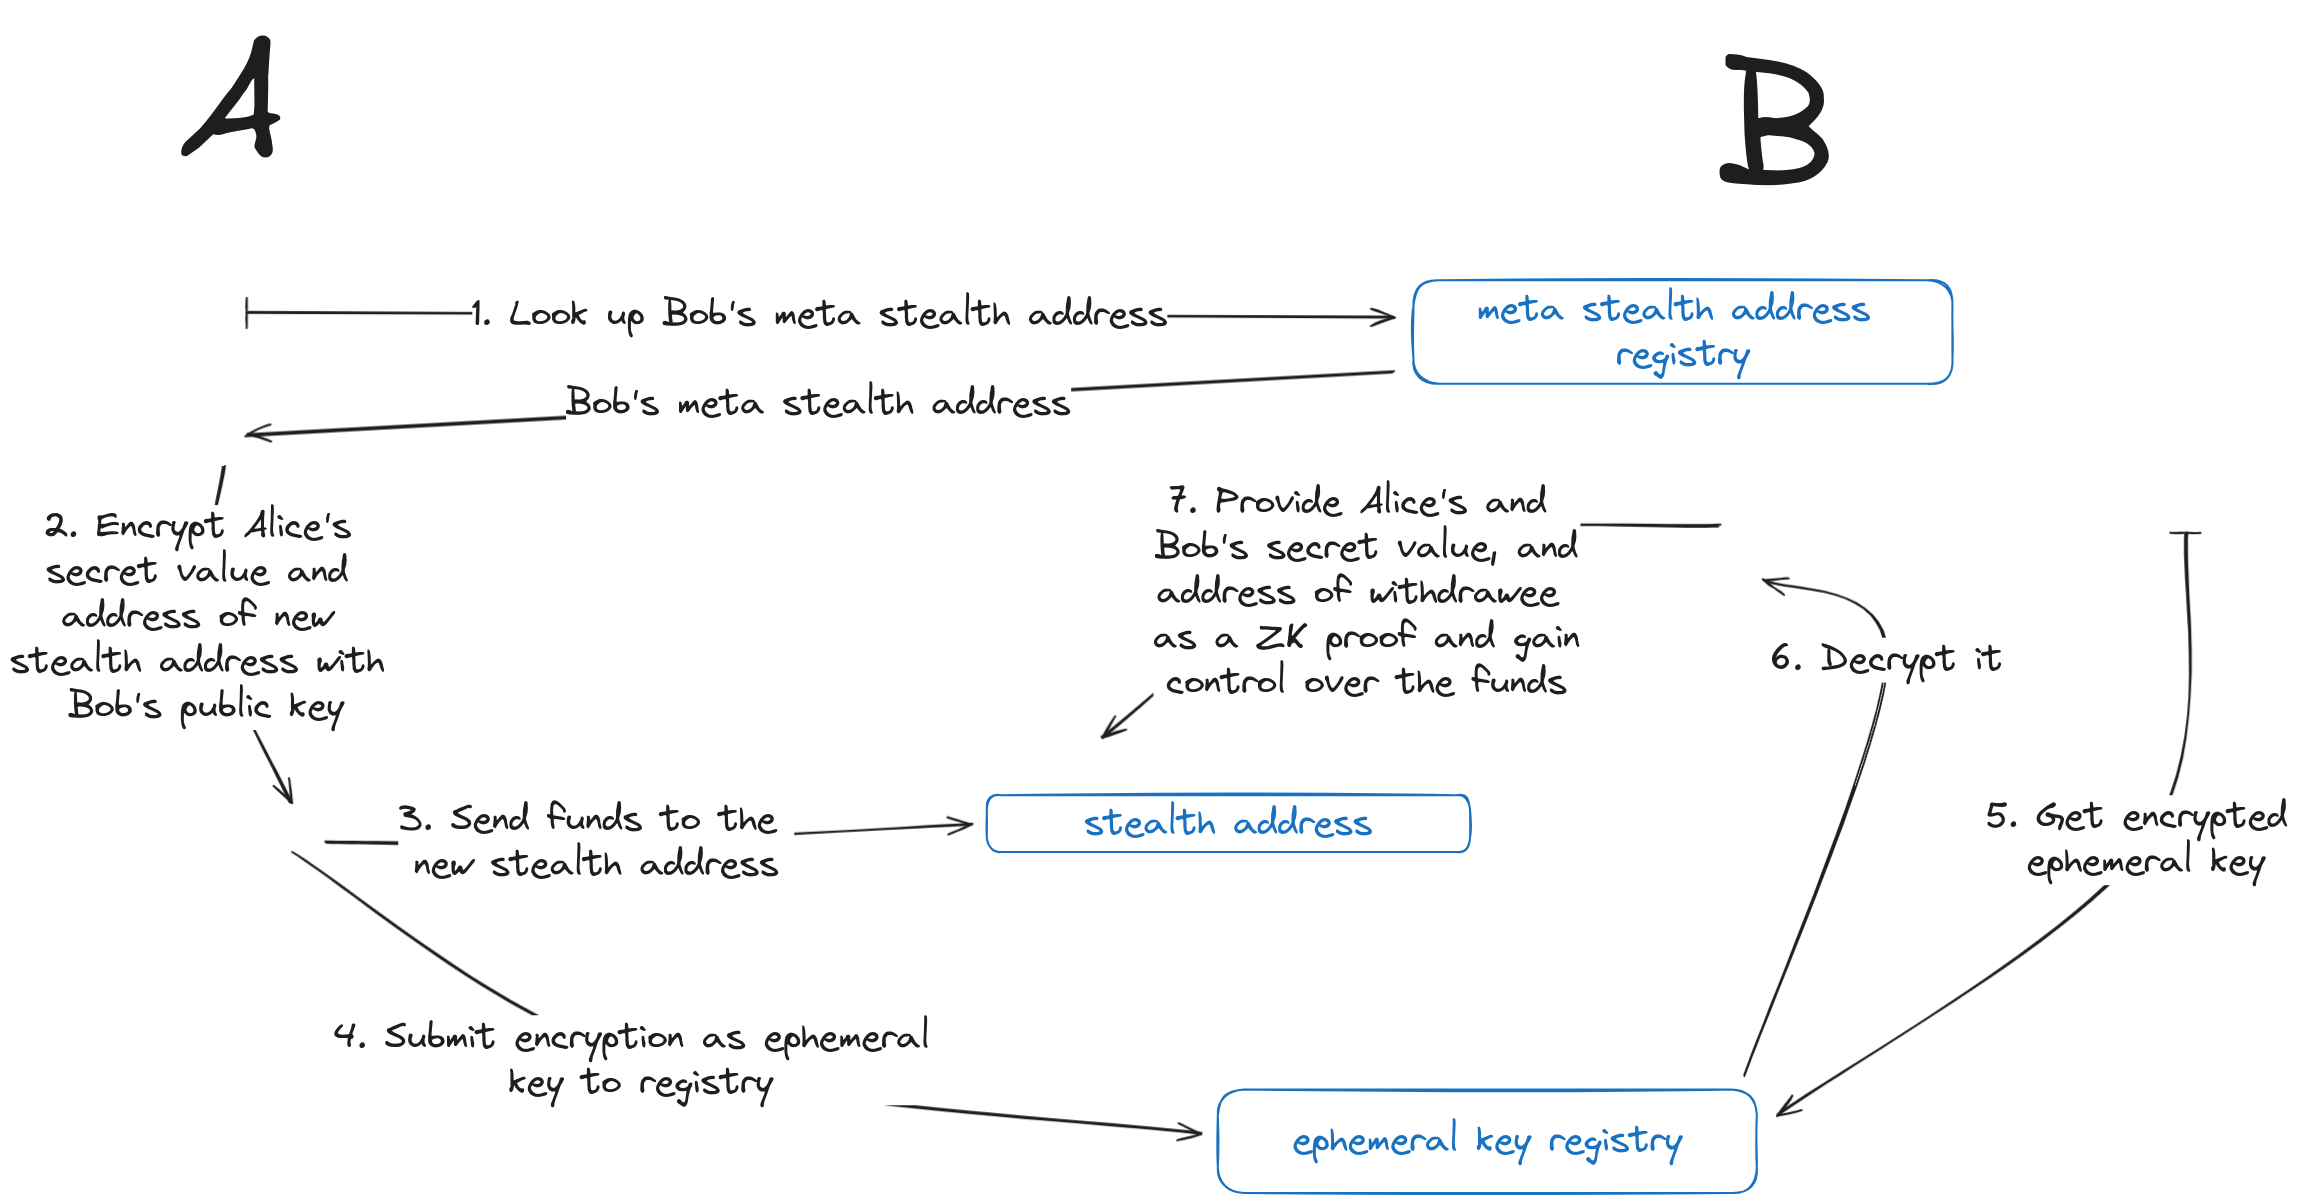
\includegraphics[scale=0.18]{assets/images/high-level.png}
    \caption{High Level Overview}
    \label{fig:hig-level}
    \vspace{0.5cm}
\end{figure}

\pagebreak
\section{Initial Setup}

Before Alice can send funds to Bob, Bob must first publish his meta stealth
address to some public location. Bob computes the following:

\begin{itemize}
	\item A private key $k$,
	\item A corresponding public key $K$,
	\item A secret value $x$,
	\item A hash of the secret value $h = hash(x)$.
\end{itemize}

Bob then publishes his meta stealth address in the form of a tuple $(K, h)$.

\begin{figure}[h]
    \centering
    
\includegraphics[scale=0.30]{assets/images/initial-setup.png}
    \caption{Initial Setup}
    \label{fig:initial-setup}
	\cite{ButerinIncompleteGuide}
    \vspace{0.5cm}
\end{figure}

\section{Sending Funds}

When Alice wishes to send funds to Bob, she queries meta stealth address registry
for Bob's meta stealth address $(K, h)$ and does the following:

\begin{itemize}
	\item Generate random secret value $c$,
    \item precompute address of the stealth address contract $sa$ \cite{stackexchangeAddressEthereum},
	\item compute $code = hash(h, c)$,
    \item deploy new stealth wallet contract with code in it,
    \item fund the deployed contract,
	\item encrypt ephemeral key $ek = encrypt(value=[c, sa], key=K)$,
    \item submit the ephemeral key to registry.
\end{itemize}

\begin{figure}[h]
    \centering
    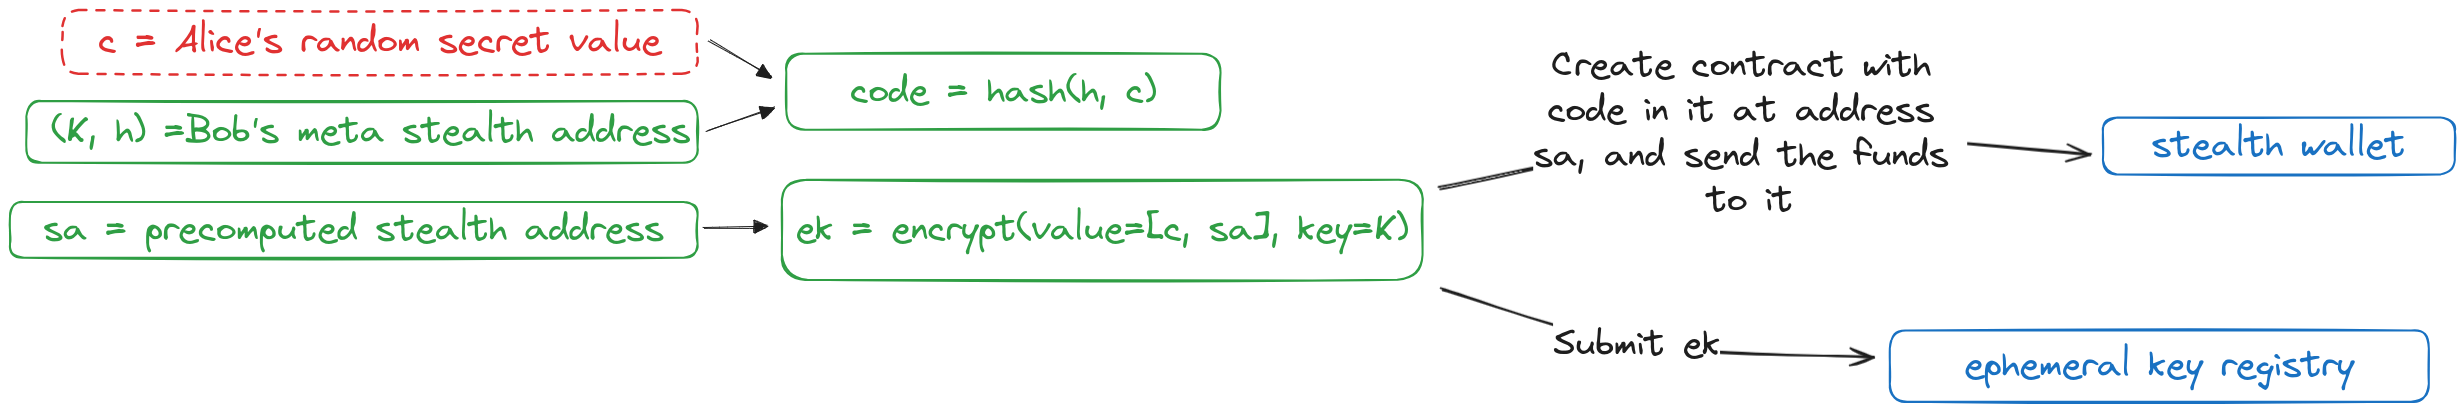
\includegraphics[scale=0.18]{assets/images/sending-funds.png}
    \caption{Sending Funds}
    \label{fig:sending-funds}
	\cite{ButerinIncompleteGuide}
    \vspace{0.5cm}
\end{figure}

\section{Scanning ephemeral keys}

Bob queries ephemeral key registry for keys from the last point he scanned.
The registry contract returns a list of ephemeral keys. Bob then tries to decrypt
each ephemeral key with his private key $k$. If the ephemeral key is meant for
Bob, then the decryption will succeed, and the decrypted value will contain
the secret value $c$ from Alice and the stealth address $sa$.

\begin{figure}[h]
    \centering
    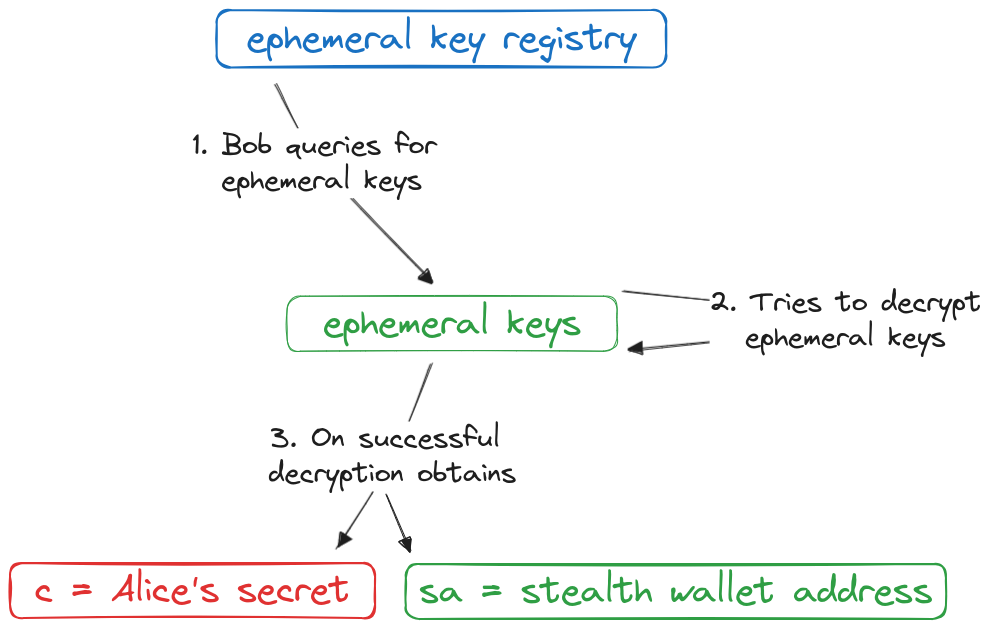
\includegraphics[scale=0.3]{assets/images/ephemeral-keys.png}
    \caption{Scanning ephemeral keys}
    \label{fig:scanning-ephemeral-keys}
    \vspace{0.5cm}
\end{figure}

\section{Gaining control of Stealth Addresses}

Bob can gain control of the stealth address $SA$ by proving to the stealth
address contract that he is the owner of the values $x$ and $c$, such that\\
$C = hash(h, c) = hash(hash(x), c)$. Bob does this by computing a ZKP for 
this statement and sending it in a transaction from any address (preferably
not from any Bob's publicly known addresses) to the stealth address $SA$. The
$SA$ contract verifies the proof and if it isn't valid, the transaction is
rejected.

\section{Overview}

The whole solution design is illustrated in Figure \ref{fig:solution},
and was inspired by the work of Vitalik Buterin \cite{ButerinIncompleteGuide}.

\begin{figure}[h]
    \centering
    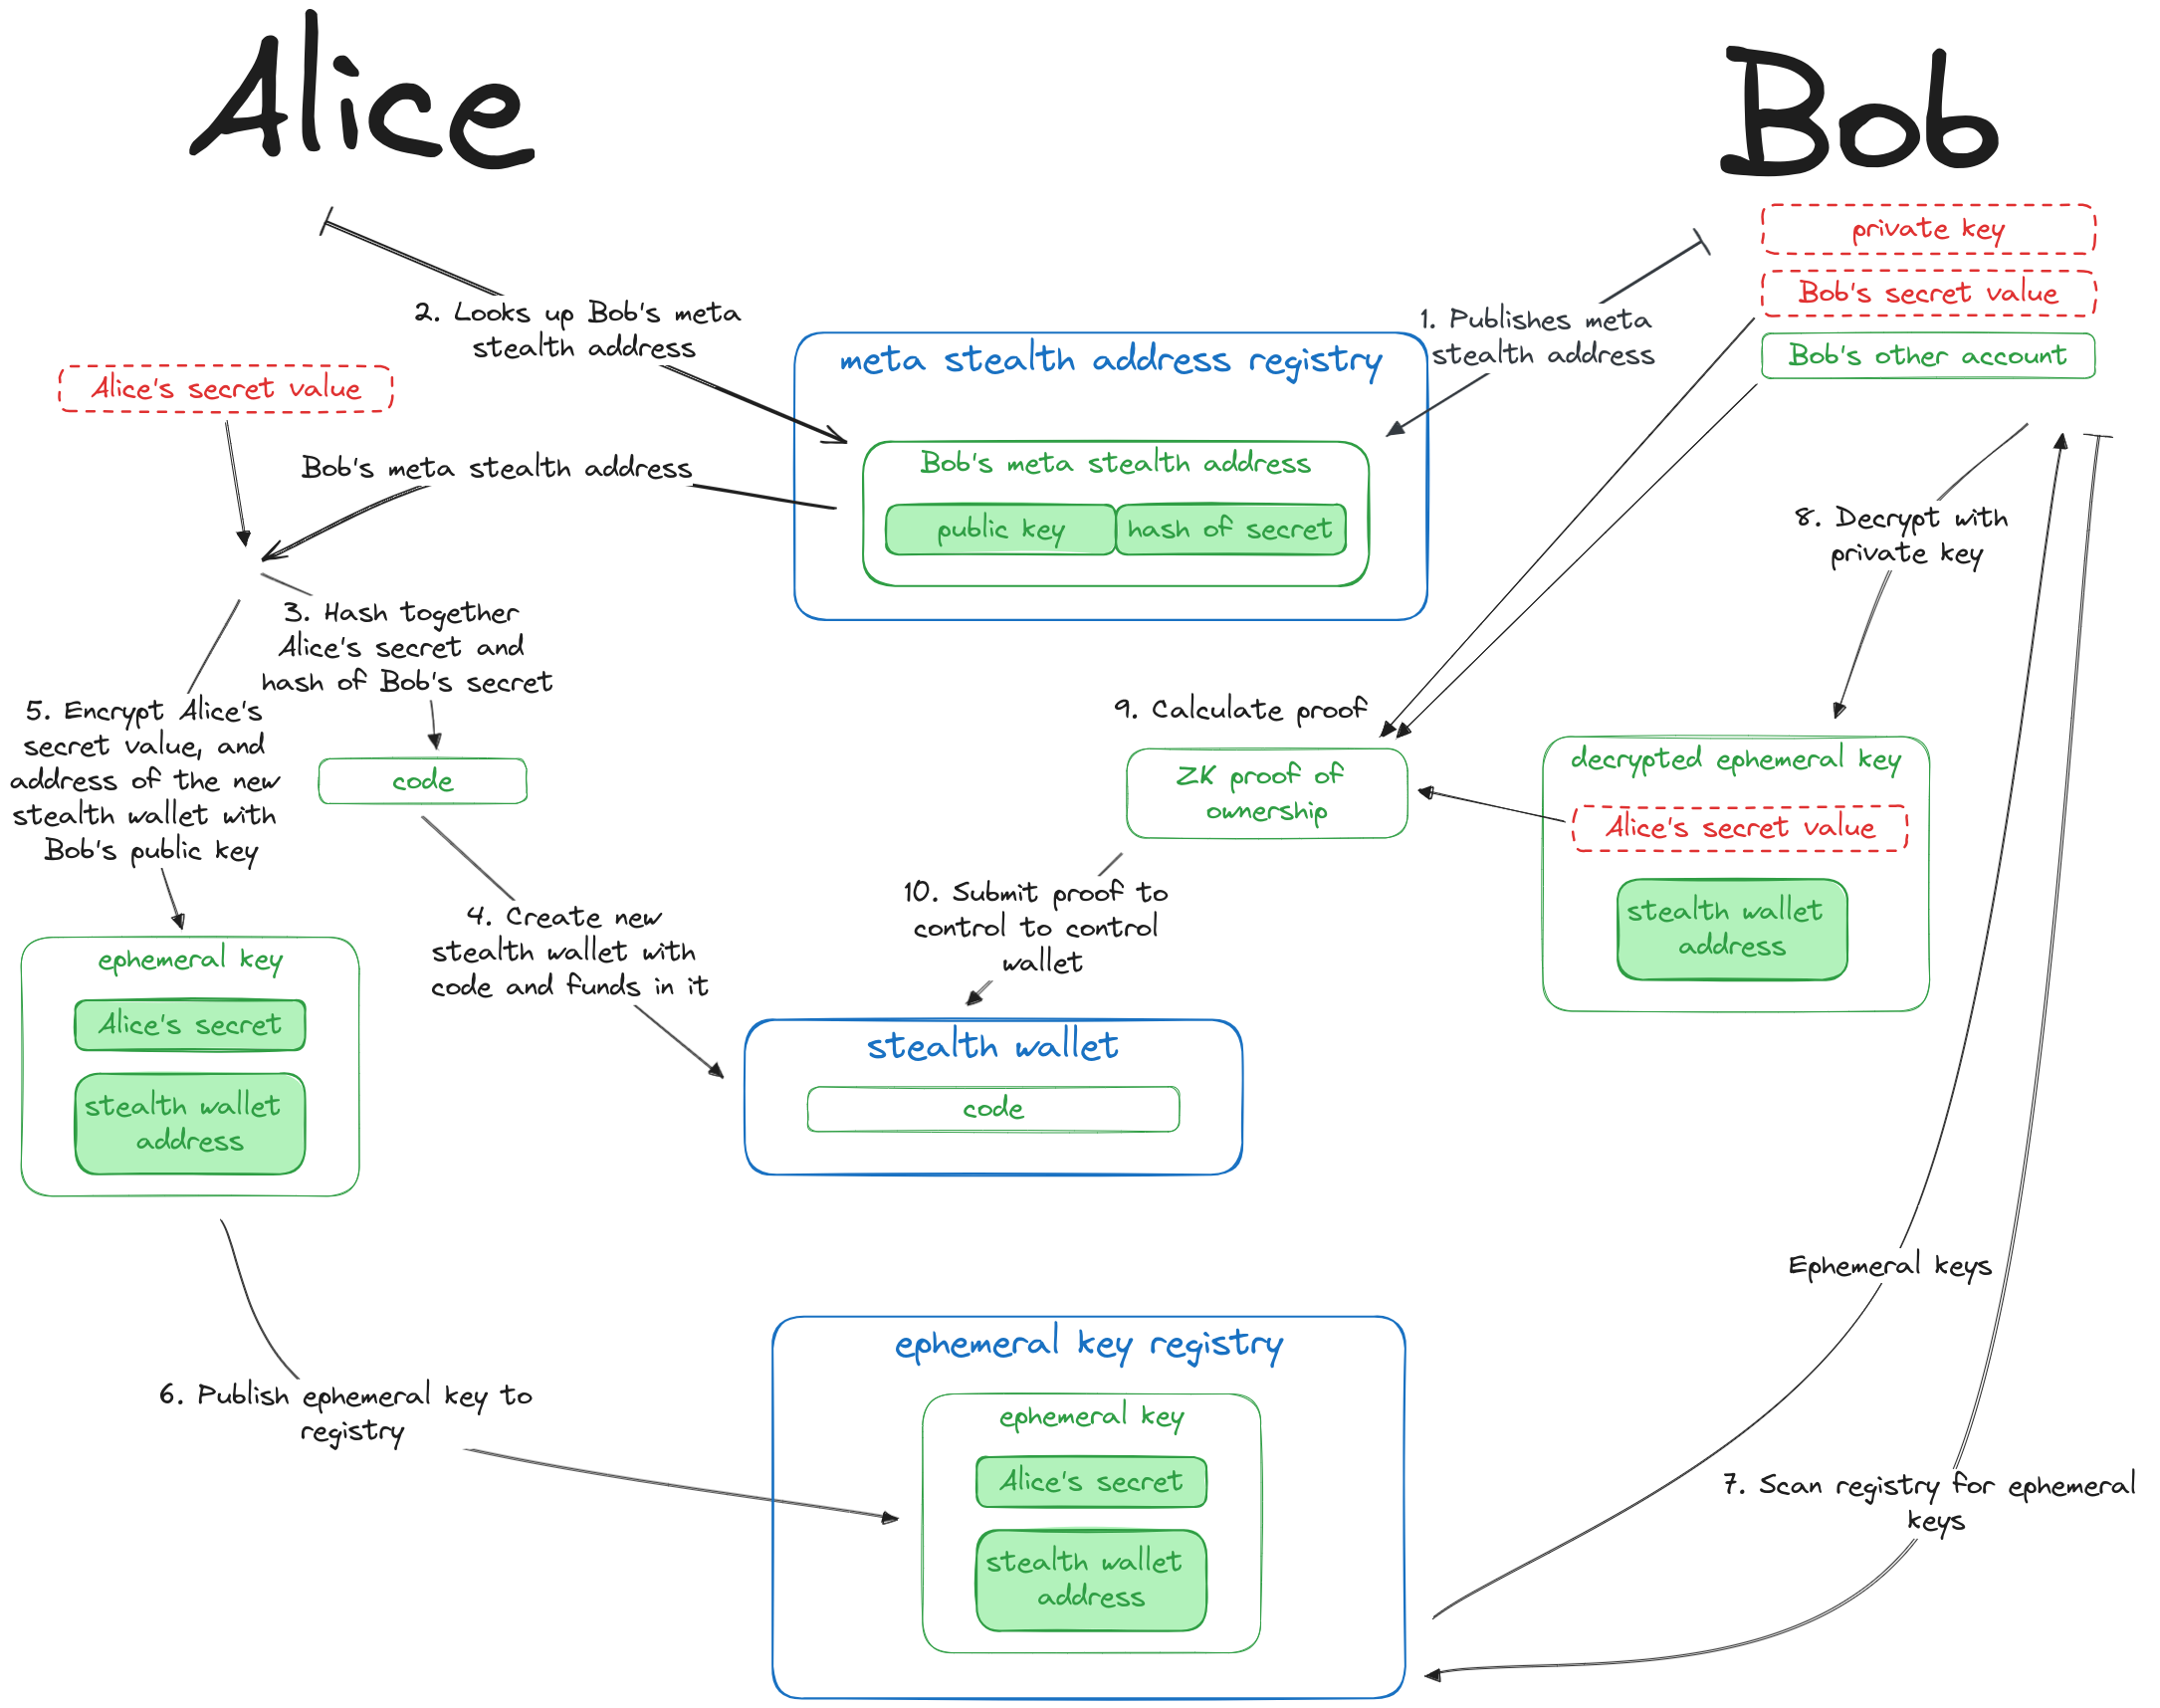
\includegraphics[width=\textwidth]{assets/images/high-level-flow.png}
    \caption{Solution Design}
	\cite{ButerinIncompleteGuide}
    \label{fig:solution}
    \vspace{0.5cm}
\end{figure}


    %
    % \chapter{Discussion on security}\label{chapter:security}

In this chapter, the security of the Stealth Address ZKP Scheme is informally discussed.

\section{Assumptions}

The security of the stealth address scheme relies on several key assumptions.
These include the security of the Groth16 ZK-SNARK system, the integrity of
the trusted setup process, the collision resistance of the hash function, the
robustness of the elliptic curve cryptography used, and the
confidentiality of the recipient's and sender's secret values. These
assumptions and consequences in a case of their falsehood are explained in next
subsections.


\subsection{Groth16}

It is assumed that the pairing-based ZK-SNARK system Groth16 \cite{Groth16} has these properties:
\begin{enumerate}
    \item Completness - honest prover will always convince honest verifier
    \item Soundness - dishonest prover will not convince honest verifier
    \item Zero Knowledge - dishonest verifier will learn nothing more then the truth of the given proposition
\end{enumerate}

If the completness property would not hold, Bob could be locked out of his stealth
addresses, because he could not prove to them that he possessed both secrets.

If the soundness would not hold, adversary could forge a false proof, which
would be verified as true, and thus could gain access to Bob's assets on given
stealth address.

And finally, if the zero knowledge property would not hold, an adversary could
learn Bob's identity, hence it would no longer be a stealth address.

\subsection{Trusted Setup}

The setup phase of Groth16 \cite{Groth16} includes a trusted setup in order to generate
public parameters. The premise of the trusted setup is that the original parameters
used to create the public ones are thrown away, if not then the party which
produced public parameters can forge false proofs, yet the verifier would
recognize them as valid ones.

In context of this work, if a party creating the circuit didn't delete the
original parameters, then it could prove malicious statements about ownership
of the secret values needed to gain control over any stealth address.

\subsection{Collision resistant hash function}\label{crhf}

First assumption is that, the used instantiation of a hash function (\textit{H})
is a collision resistant one. Meaning it is computationally hard to find two
inputs \textit{a}, \textit{b}, such that

\[ a \neq b \land H(a) = H(b) \]

Otherwise, an adversary could, for example, find a value $x^\prime$,
such that Bob's secret value $x$ and $x^\prime$ are not equal, but their hashes
are. Then the $x^\prime$ could be used to gain control over Bob's stealth address,
if the adversary knew Alice's secret value, or in the case when Alice is a malicious
actor, she could send assets to Bob's stealth address, but with $x^\prime$ and
her secret value, could withdraw them without any public proof that she did it.

As showcased earlier, this vulnerability alone is not enough to gain control
over Bob's stealth address, adversary also must know Alice's secret value to
gain control over a Bob's stealth address, but only the one she interacted with.

Also, if used hash function is not a collision resistant one, adversary still can not
discover the identity of Bob, or any of his other stealth addresses.

\subsection{Elliptic Curve Crypthography - Secp256k1}

Next assumption is that the Secp256k1 elliptic curve parameters used in Ethereum
and Bitcoin \cite{bitcoinSecp256k1Bitcoin} are well-chosen and do not contain any backdoors. Additionally, it is
assumed that advancements in cryptographic research and technology do not
compromise the security of Secp256k1.

If not, an adversary could recover Bob's private key and decrypt all of his
ephemeral keys submitted to the Ephemeral Key Registry contract. The
adversary would know all Bob's stealth addresses and, also have all secret
values used to create codes in those stealth addresses. However, with this
vulnerability alone, the adversary can not control Bob's stealth addresses,
because he/she is missing the Bob's secret value $x$.

\subsection{Knowledge of recipient's secret value}

If an adversary somehow learns Bob's secret value $x$, he/she does not have enough
information to control any of Bob's stealth addresses. On the other hand, if Alice,
or any other sender, would learn Bob's secret value $x$, she could, as in the
\ref{crhf} steal Bob's assets from the stealth address she interacted with and
Bob would not have any public proof that it was her.

\subsection{Knowledge of sender's secret value}

If an adversary somehow learns Alice's secret value $c$, the corresponding
address is still safe, because, the attacker does not know which stealth address
it is, and if somehow learned it, he/she still does not have Bob's secret value.

\section{Discussion summary}

Given these assumptions, the presented Stealth Address ZKP Scheme can be used to
send assets to a recipient, without leaking any information about him/her. And
guarantees to the recipient that only he/she has access to stealth addresses.


    %
    % \chapter{Implementation}\label{chapter:implementation}

In this section different terminology is used, instead of Bob, owner is used,
and instead of Alice sender is used. The implementation of this study is
separated into 3 modules (depicted in \ref{fig:component-diagram}), module for the
circuit which will compute ownership proofs, another one for smart contracts
needed to implement stealth wallet with ZKP stealth address schema, and
module with a web app wallet client used to interact with the stealth wallets.

The implementation is only a proof of concept, not a full featured wallet.
The sender's part is the same as described until now. The owner however,
can only withdraw all funds from the wallet into another address. This does
not detract from demonstrating the core concept of a ZKP stealth address schema.
Fractional withdrawals, ERC20 token transfers, transaction proxying and other wallet
features can be implemented in future work.

\begin{figure}[h!]
    \centering
    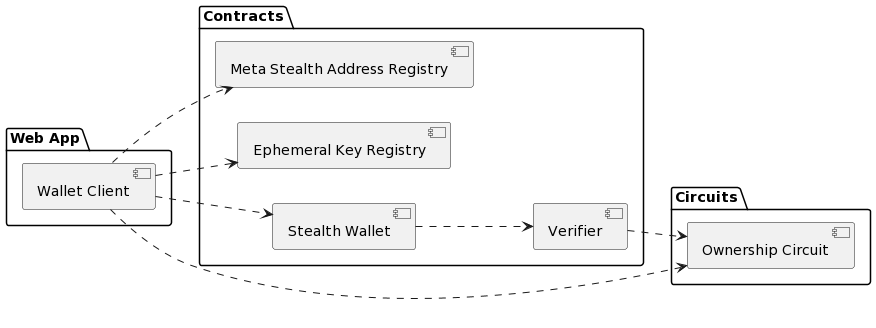
\includegraphics[width=\textwidth]{assets/images/component-diagram.png}
    \caption{Component diagram}
    \label{fig:component-diagram}
    \vspace{0.5cm}
\end{figure}

\section{Interaction between components}

The interaction between components, and users is depicted in Figure \ref{fig:component-diagram}.

\begin{figure}[h!]
    \centering
    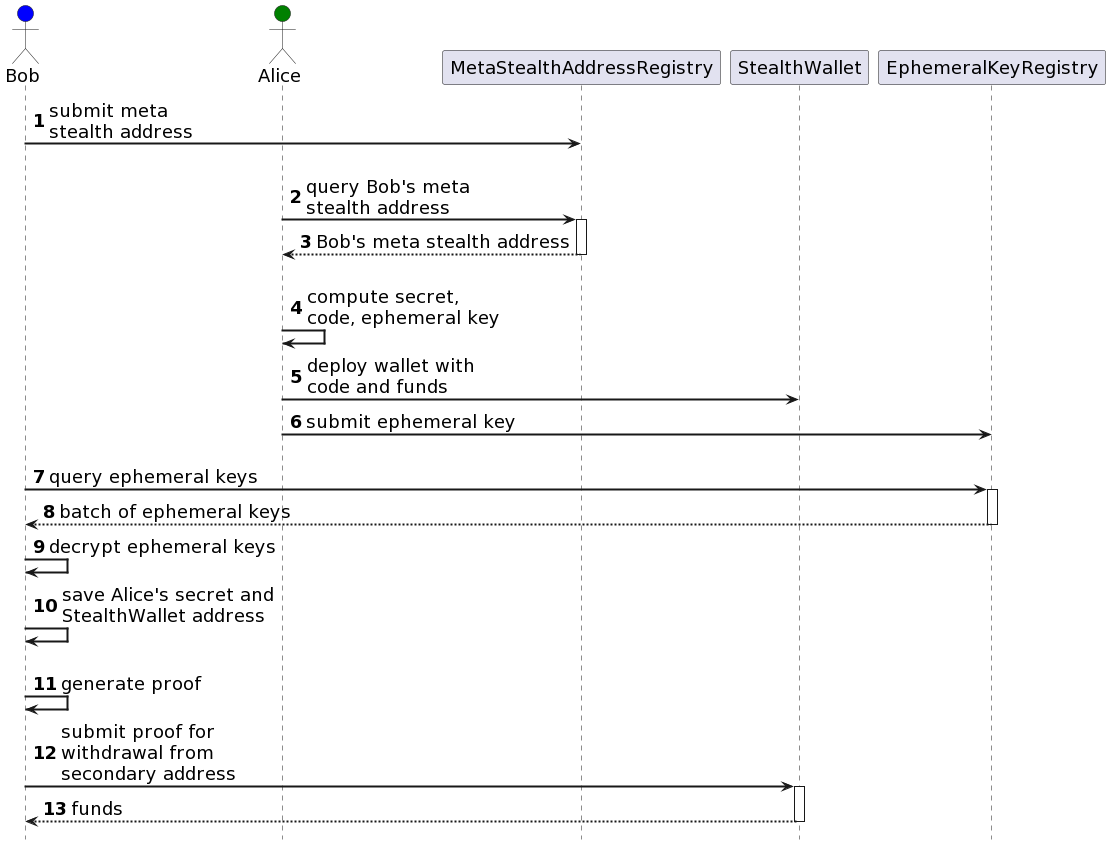
\includegraphics[width=\textwidth]{assets/images/implementation-flow.png}
    \caption{Interaction flow}
    \label{fig:interaction-flow}
    \vspace{0.5cm}
\end{figure}


\section{Circuits}

Circuits for proving and verifying ZKPs are written in Circom 2 \cite{circomCircomDocumentation}.
With circom compiler, a circuit is compiled into a Groth16
ZK-SNARK proof system \cite{Groth16} representation. Circom also generates
either C++ of Wasm source files for computing witness (proof) for the
circuit. Circuit written in this study, which proves ownership, has
these private inputs:
\begin{enumerate}
    \item owner's secret value,
    \item sender's secret value,
    \item and the withdrawee address.
\end{enumerate}
And these public inputs:
\begin{enumerate}
    \item code that was submitted by sender on contract creation,
    \item and the transaction sender.
\end{enumerate}

Groth16 requires a trusted setup for each circuit. For Groth16 trusted
setup, there are two parts:
\begin{enumerate}
    \item Powers of Tau ceremony \cite{PowersOfTau},
    \item and phase 2 dependent on the circuit.
\end{enumerate}
Powers of Tau ceremony is used to generate initial parameters for a SNARK.
In this ceremony, the initial parameters are generated using a multi-party
computation. If only one party in this computation is acting honestly,
the entire process is trustworthy and the initial parameters are secure
for use with any circuit. There is ongoing public powers of tau ceremony
called Perpetual Powers of Tau \cite{PerpetualPTAU}. Its goal is to
securely generate SNARK parameters for circuits. In this study a powers
of tau ceremony file from SnarkJS \cite{snarkjs} is used, which is from
this ceremony. Phase 2 is generated with SnarkJS and is specific for circuit.

\section{Smart contracts}

Smart contracts in this implementation are written in programming
language Solidity \cite{solidity} and are developed and tested
with Foundry \cite{foundry}. They are deployed through
Infura \cite{infura} Ethereum RPC provider to the Sepolia Ethereum
testnet \cite{sepolia}.

There are four smart contracts implemented. A meta stealth address
registry which holds meta stealth addresses. A ephemeral key registry
which holds the ephemeral keys. A verifier of previously mentioned
circuit. And contract for the stealth wallet.

Owners submit their meta stealth addresses to meta stealth address registry,
and senders query it for them. To the ephemeral key registry senders submit
ephemeral keys and owners query it for them. Senders deploy stealth wallets
with funds and computed codes. Owners send proofs to stealth wallets,
which interact with the verifier.

This module also contains tests. Code coverage report for these is shown in
table \ref{table:coverage}.

\begin{table}[ht]
\centering
\scalebox{0.7}{
    \begin{tabular}{l | r r r r}
    \toprule
        \textbf{File} & \textbf{\% Lines} & \textbf{\% Statements}  & \textbf{\% Branches}  & \textbf{\% Funcs} \\ 
        \midrule
        script/DeployConfig.s.sol  & 0.00\% (0/5)    & 0.00\% (0/7)     & 0.00\% (0/2)     & 0.00\% (0/3)   \\
        script/DeployContracts.s.sol & 0.00\% (0/7)    & 0.00\% (0/9)     & 100.00\% (0/0)   & 0.00\% (0/1)   \\
        src/EphemeralKeyRegistry.sol & 92.86\% (13/14) & 94.44\% (17/18)  & 66.67\% (4/6)    & 66.67\% (2/3)  \\
        src/MetaStealthAddressRegistry.sol & 100.00\% (8/8)  & 100.00\% (11/11) & 100.00\% (4/4)   & 100.00\% (2/2) \\ 
        src/StealthWallet.sol  & 91.67\% (11/12) & 92.31\% (12/13)  & 83.33\% (5/6)    & 66.67\% (2/3)  \\
        src/Verifier.sol   & 100.00\% (0/0)  & 100.00\% (0/0)   & 100.00\% (0/0)   & 100.00\% (1/1) \\
        \midrule
        \textbf{Total} & 69.57\% (32/46) & 68.97\% (40/58)  & 72.22\% (13/18)  & 53.85\% (7/13) \\
        \bottomrule
        \end{tabular}
}
\caption{Solidity code coverage}
\label{table:coverage}
\end{table}

The first two files are not covered, because they only contain simple logic
for deploying contracts and do not interfere in any functionality of the
implemented stealth address scheme.

\section{Web app}

Browser wallet client used to interact with stealth wallets is written in
frontend framework SolidJS \cite{solidjs}, with Web3JS \cite{web3js}
as the main library for interacting with blockchain, and Infura \cite{infura}
is used as a Ethereum RPC provider.

It consists of two sub-pages, one for sender (Alice), in which a sender
can query meta stealth addresses and deploy stealth wallets only accessible
by the owners of corresponding meta stealth addresses. And the second one,
for owners (Bob) which displays all stealth wallets with balance and enables
owners to withdraw funds from them by generating ZKPs.


    %
    % \chapter{Evaluation}\label{chapter:evaluation}

\section{Requirement satisfaction}

How the implementation of the stealth address scheme, as detailed in Chapter
\ref{chapter:implementation}, fulfills the functional requirements outlined in
the Chapter \ref{chapter:solution}, can be seen in Figure \ref{fig:usecase-diagram}.

\begin{figure}[h!]
    \centering
    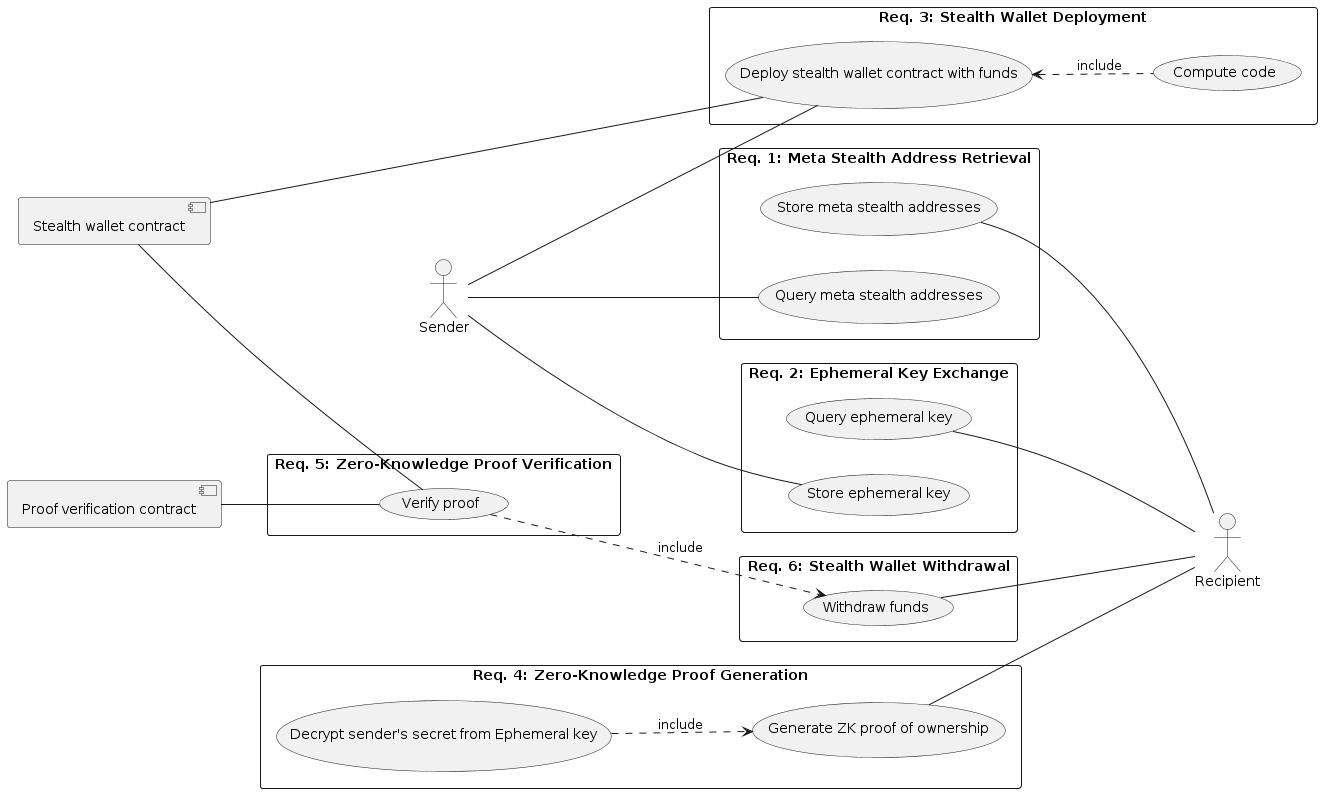
\includegraphics[width=\textwidth]{assets/images/usecase-diagram.png}
    \caption{Usecase diagram}
    \label{fig:usecase-diagram}
    \vspace{0.5cm}
\end{figure}
\pagebreak

\section{Demonstration on Sepolia Testnet}

This section walks through a demonstration of the ZKP stealth address scheme
deployed on Sepolia testnet. For this demonstration, this will be Alice's
address \href{https://sepolia.etherscan.io/address/0x2668Bc59Fa9001DBBA2bD255Bf24b9Fc8c1AbAd7}{0x2668Bc59Fa9001DBBA2bD255Bf24b9Fc8c1AbAd7}
this is Bob's primary address
\href{https://sepolia.etherscan.io/address/0x1c6Ff1028E166C9D4A15a5a019041077793c64D3}{0x1c6Ff1028E166C9D4A15a5a019041077793c64D3}
and this is Bob's second address
\href{https://sepolia.etherscan.io/address/0xc86B622175eDd2274d374dD86e13Ba521e4B876b}{0xc86B622175eDd2274d374dD86e13Ba521e4B876b}.

Both Alice's and Bob's secondary addresses have one transaction each, which were
only used to fund the address with some Ether for this demonstration.
These transactions are disregarded in this demonstration.
Bob's primary address contains one funding transaction, and two transactions
which were used to setup Bob's meta stealth address (the first transaction was
a mistake, that is why there are two). The initial state of both Alice and Bob
are shown in figure \ref{fig:alice-initial} and \ref{fig:bob-initial} respectively.

The address of the meta stealth address registry is\\
\href{https://sepolia.etherscan.io/address/0xa08aaf964300121f6c1bd962f7b53c7e06d909bd#code}{0xa08AaF964300121f6C1bD962f7B53C7e06d909BD}
and the address of the ephemeral key registry is
\href{https://sepolia.etherscan.io/address/0x156bcce17d7409a32c408e2aab8f04c8cbd7c450}{0x156Bcce17d7409A32C408e2AAb8F04C8CBd7c450}.

\begin{figure}[h!]
    \centering
    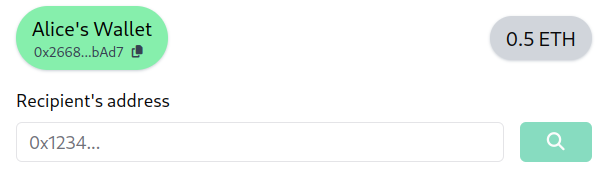
\includegraphics[width=\textwidth]{assets/images/demo/alice-initial.png}
    \caption{Initial state of Alice's wallet}
    \label{fig:alice-initial}
\end{figure}

\begin{figure}[h!]
    \centering
    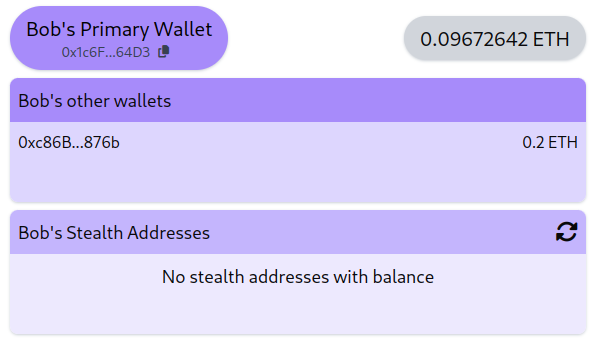
\includegraphics[width=\textwidth]{assets/images/demo/bob-initial.png}
    \caption{Initial state of Bob's wallet}
    \label{fig:bob-initial}
\end{figure}

Alice can paste Bob's primary address and query the meta stealth address
registry for his meta stealth address, shown in figure \ref{fig:meta-query}.

\begin{figure}[h!]
    \centering
    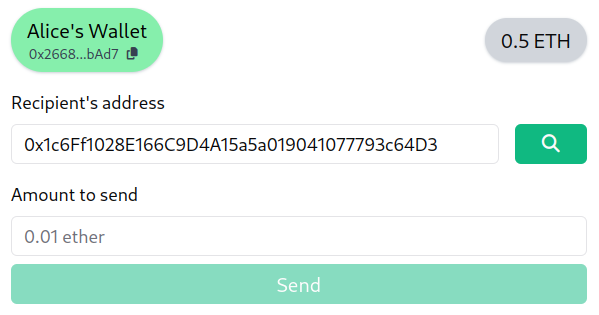
\includegraphics[width=\textwidth]{assets/images/demo/meta-query.png}
    \caption{Querying Bob's meta stealth address}
    \label{fig:meta-query}
\end{figure}

Figure \ref{fig:meta-not-found} displays scenario when Alice queries for an
address without meta stealth address.

\begin{figure}[h!]
    \centering
    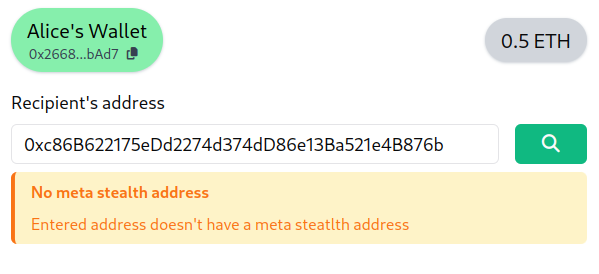
\includegraphics[width=\textwidth]{assets/images/demo/meta-not-found.png}
    \caption{Querying address without meta stealth address}
    \label{fig:meta-not-found}
\end{figure}

\pagebreak
When Alice sends funds to Bob's stealth address, she first 
\href{https://sepolia.etherscan.io/tx/0xabac631e68de9c31a4cf00d55328b9a35fff55f6baf475849197415c62b1d394}{deploys},
the stealth wallet contract and then 
\href{https://sepolia.etherscan.io/tx/0xce4a7169458a1e09ee027645c833a9a16a0ff10557a61d7fa5c3b3dabf7abee8}{submits the ephemeral key}
to the ephemeral key registry. Bob can then scan the ephemeral key registry and decrypt Alice's secret, and the
address of his stealth wallet with sent funds. Stealth wallets are then tracked,
shown in figure \ref{fig:stealth-address-tracking}.

\begin{figure}[h!]
    \centering
    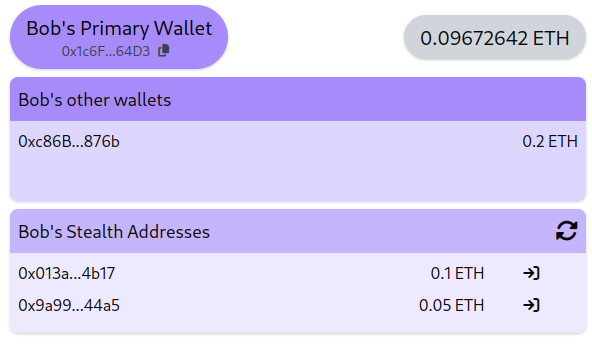
\includegraphics[width=\textwidth]{assets/images/demo/stealth-address-tracking.png}
    \caption{Tracking of Bob's stealth addresses}
    \label{fig:stealth-address-tracking}
\end{figure}

If Bob wants to use the funds, he can withdraw them to the his secondary address,
which is not linked to his primary address, as depicted in figure \ref{fig:bob-withdraw}.

\begin{figure}[h!]
    \centering
    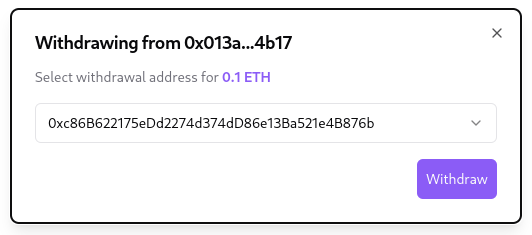
\includegraphics[width=\textwidth]{assets/images/demo/bob-withdraw.png}
    \caption{Withdrawing of funds}
    \label{fig:bob-withdraw}
\end{figure}

When accepted, the browser wallet generates a proof from Bob's secret value,
Alice's secret value and address which will be doing the withdrawal. The
proof is
\href{https://sepolia.etherscan.io/tx/0x78fabcfe3a78a7453cbe63c3f64340e80610fe6d5ceda8c250687facc52981a2}{submitted}
and funds are transferred to the chosen withdrawal address, as shown in figure \ref{fig:after-withdrawal}.

\begin{figure}[h!]
    \centering
    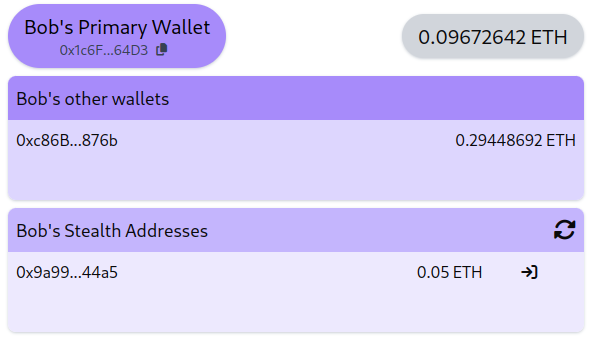
\includegraphics[width=\textwidth]{assets/images/demo/after-withdrawal.png}
    \caption{State of Bob's secondary address after withdrawal}
    \label{fig:after-withdrawal}
\end{figure}

\section{Gas analysis}

The gas consumption of the smart contracts was analyzed using the \texttt{forge test --gas-report}
command, which is part of the Foundry development framework. The most important
gas metric is the one for withdrawing funds from StealthWallet contract,
because in that function the proof validation occurs. The median for it
is \texttt{223902} gas, little higher than a Uniswap V3 swap.
The gas cost of the withdrawal function is dominated by the proof verification, which is done by
the \texttt{verifyProof} function in the \texttt{Groth16Verifier} contract. This function has a
constant gas cost of \texttt{195686}. The remaining gas is used for other operations
in the withdrawal function, such as transferring funds to the recipient.

\begin{table}[H]
    \centering
    \begin{tabular}{|l|r|r|r|r|r|}
        \hline
        \textbf{EphemeralKeyRegistry} &  &  &  &\\
        \hline
        Deployment Cost & Deployment Size &  &  &\\
        400998 & 1642 &  &  &\\
        \hline
        Function & min & avg & median & max\\
        \hline
        getKeysBatch & 423 & 4340 & 4920 & 10612\\
        submit & 58133 & 160677 & 161129 & 178229\\
        \hline
    \end{tabular}
\end{table}

\begin{table}[H]
    \centering
    \begin{tabular}{|l|r|r|r|r|r|}
        \hline
        \textbf{MetaStealthAddressRegistry} &  &  &  &\\
        \hline
        Deployment Cost & Deployment Size &  &  &\\
        501153 & 2107 &  &  &\\
        \hline
        Function & min & avg & median & max\\
        \hline
        addressMetaStealthAddress & 1956 & 3105 & 1956 & 5404\\
        setMetaStealthAddress & 25346 & 60353 & 36146 & 119051\\
        \hline
    \end{tabular}
\end{table}

\begin{table}[H]
    \centering
    \begin{tabular}{|l|r|r|r|r|r|}
        \hline
        \textbf{Groth16Verifier} &  &  &  &\\
        \hline
        Deployment Cost & Deployment Size &  &  &\\
        371621 & 1506 &  &  &\\
        \hline
        Function & min & avg & median & max\\
        \hline
        verifyProof & 195686 & 195686 & 195686 & 195686\\
        \hline
    \end{tabular}
\end{table}

\begin{table}[H]
    \centering
    \begin{tabular}{|l|r|r|r|r|r|}
        \hline
        \textbf{StealthWallet} &  &  &  &\\
        \hline
        Deployment Cost & Deployment Size &  &  &\\
        268322 & 1257 &  &  &\\
        \hline
        Function & min & avg & median & max\\
        \hline
        withdraw & 23100 & 182078 & 223902 & 257409\\
        \hline
    \end{tabular}
\end{table}

\section{Static analysis}

The implementation of the smart contracts was analyzed using the static analyzers
Aderyn \cite{githubCyfrinaderyn} and Slither \cite{githubCryticslither}.

\subsection{Aderyn results}

Static analysis of the smart contracts using the Aderyn tool revealed four low-severity issues.

\begin{enumerate}
    \item \textbf{Imprecise Solidity Pragma:} The use of a broad Solidity
        pragma \texttt{\textasciicircum0.8.13} was flagged, suggesting the use of a specific version for
        better compatibility and security. This was addressed by changing the
        pragma to pragma solidity 0.8.20;
    \item \textbf{Missing Zero Address Check:} The \texttt{StealthWallet.sol}
        lacked a check for the zero address of a verifier contract. This was
        fixed by adding the necessary check.
    \item \textbf{Public Function Optimization:} Some public functions that
        were not used internally were identified as potential candidates for being
        marked as external to optimize gas usage. These functions were modified
        accordingly.
    \item \textbf{PUSH0 Opcode Compatibility:} The report noted that the
        Solidity compiler version used could generate bytecode with PUSH0 opcodes,
        which might not be supported on all (EVM) chains.
        This was acknowledged, and it was decided to deploy the contracts only on
        chains that support EVM Shanghai, which includes the PUSH0 opcode.
\end{enumerate}

The whole report generated by Aderyn can be found in\\\texttt{stealth-wallet/aderyn-report.md}.

\subsection{Slither results}

Static analysis of the smart contracts using Slither identified several
issues, categorized as high, low, informational, and optimization.
However, it is important to note that the majority of these findings were in the
generated \texttt{Verifier.sol} contract and external library code, rather
than the core logic of the implemented stealth address scheme.

\subsubsection*{High Severity}
\begin{enumerate}
    \item \textbf{arbitrary-send-eth:} When withdrawing from stealth wallet, Ether
        could potentially be sent to an arbitrary address due to the lack of
        validation on the recipient's address in the withdraw function. This is
        not true, since only a owner can generate a valid proof, so funds
        will be transfered to address specified by the owner.
    \item \textbf{incorrect-return:} Three instances of incorrect return
        values were identified in the Groth16Verifier contract, which could halt
        execution. This contract is generated with SnarkJS, hence these issues
        can only be acknowledged. Fixing these issues in the SnarkJS generator
        is outside the scope of this project.
\end{enumerate}

\subsubsection*{Low Severity}
\begin{enumerate}
    \item \textbf{missing-zero-check: } Stealth wallet did not check if the
        recipient address is zero address, this check was added.
\end{enumerate}

\subsubsection*{Informational}
Several informational findings were related to the use of assembly code,
pragma directives, Solidity compiler versions, low-level calls, naming
conventions, and unused state variables. These were primarily found in the
generated \texttt{Verifier.sol} contract and external library code. While acknowledged,
they were not considered to directly impact the security or functionality of
the implemented scheme.

\subsubsection*{Optimization}
Two state variables in the stealth wallet contract were identified as potential
candidates for being declared as immutable, which could optimize gas usage.
These variables were made immutable.

The whole report generated by Slither can be found in\\\texttt{stealth-wallet/slither-report.md}.

    %
    % \chapter{Conclusion}\label{chapter:conclusion}

This thesis has presented how ZKPs can be applied to the problem of stealth
addresses in Ethereum. How one can receive payments without revealing their
identity, and do so without the need to actively communicate with the sender.

This proof of concept of a ZKP Stealth address Scheme on Ethereum allows
a sender to send funds to a recipient without any prior communication, and
without submitting any data, that links the sender with the recipient, to the blockchain.
And allows the recipient to prove that they are the intended recipient of the
funds, without revealing their identity, and without the need to actively
communicate with the sender.

The key novelty and scientific contribution of this work lie in the successful
demonstration of the practical application of ZKPs to address real-world
privacy challenges in blockchain technology. By presenting a conceptual
implementation of the stealth address scheme, this thesis showcases the
potential of ZKPs to enhance privacy and security in blockchain-based
applications. The scheme's design allows for the creation of stealth addresses
that are not directly linked to the recipient's identity, while still enabling
the recipient to prove ownership and control over the funds. This
proof-of-concept implementation serves as a contribution to the
ongoing research and development in the field of privacy-preserving blockchain
technologies.

\section{Future Work}

The design and implementation of the ZKP stealth address scheme serves only as
a proof of concept. For this scheme to be widely adopted, additional work is
required. This chapter outlines some of the potential future work that could be
done to improve the scheme.

\subsection*{Ephemeral Key Search}

The current implementation of the ZKP stealth address scheme requires that sender
submits the ephemeral public key to a registry. The registry is just a simple
storage that stores these keys in a list. This method does not scale well with
mass adoption. Each recipient would have to scan the entire list of keys to
check if any belong to them.

Current ERC-5564 \cite{ethereumERC5564Stealth} proposal, which differs from
here proposed scheme mainly in the use of elliptic curve cryptography instead
of ZKPs, uses view tags to reduce the number of keys that need to be scanned.
Or, different approach, proposed by Xin Wang, Li Lin, Yao Wang \cite{Wang2023}
utilizes subgroup membership assumption related to factoring for faster key
search.

\subsection*{Recoverability}

The current implementation of the ZKP stealth address scheme does not allow for
possibility of funds recovery. This means that if the recipient loses their
private key, they will not be able to recover their funds.

One way to address this issue would be to use a private key recovery
mechanism, such as Shamir Backup. With this approach, the stealth address
scheme would not need to be modified, because the private key recovery would
be handled outside of the blockchain.

Different approach would be to modify the stealth address scheme to implement
a concept of a Social Recovery Wallet. These types of wallets enable user to
assign guardians to their wallet. Guardians are different accounts, for example
friends, mobile phone, hardware wallet or some kind of institution. The wallet
holds a public key to some user owned private key. Only this key can control
the wallet. If the user loses their private key, they can request the
guardians to change the associated public key in the wallet, thus changing the
private key that is used to control the wallet \cite{ButerinSocialRecovery}.
An incomplete implementation of this concept was proposed by Vitalik Buterin \cite{ButerinIncompleteGuide},
which uses ZKPs to prove to the stealth addresses, that the user is the owner
of the wallet.




    % \ifx\FIITlagEN\undefined
    % \else
    %     % Resume in Slovak
\thispagestyle{empty}

\begin{otherlanguage}{slovak}
\chapter*{Resumé}
\markboth{Resumé}{Resumé}
\addcontentsline{toc}{chapter}{Resumé} 

Táto bakalárska práca skúma aplikáciu dôkazov s nulovým vedomím (ZKPs) v
blockchainoch. Dôkazy s nulovým vedomím sú kryptografická metóda, ktorá
umožňuje overenie dát bez odhalenia samotných dát, čo je ideálne pre
bezpečné a súkromné aplikácie v blockchainoch.

Práca sa zaoberá riešením problému nedostatočného súkromia v
blockchainových transakciách. Blockchainy ako Ethereum ponúkajú
transparentnosť a bezpečnosť, verejná povaha transakcií odhaľuje identity
používateľov a ich finančné aktivity, čo vyvoláva značné obavy o súkromie.
Táto práca predstavuje nové riešenie tohto problému pomocou dôkazov s
nulovým vedomím na vytvorenie schémy tajných adries.

\section{Úvod}

V úvode  je predstavený koncept dôkazov s nulovým vedomím (ZKPs), čo je
kryptografická metóda umožňujúca overenie pravdivosti tvrdenia bez
odhalenia jeho obsahu. Popisuje históriu ZKPs, počnúc ich konceptom v roku
1989, a ich vývoj smerom k neinteraktívnym dôkazom. Tieto dôkazy umožňujú
overenie bez nutnosti priamej interakcie medzi stranami. Kapitola tiež
zdôrazňuje význam tajných adries v blockchainoch, ktoré umožňujú
odosielanie aktív bez odhalenia identity príjemcu. Použitie ZKPs v
kontexte tajných adries zvyšuje súkromie tým, že umožňuje príjemcovi
preukázať vlastníctvo adresy bez prezradenia svojej identity.

Analýza (\ref{chapter:analysis}) opisuje kryptografické princípy za ZKPs a
ich využitie v blockchainoch, najmä v schéme tajných adries. V kapitole
Súvisiaca práca (\ref{chapter:related}) sa skúma existujúci výskum a projekty
týkajúce sa ZKPs a tajných adries. Návrh riešenia (\ref{chapter:solution}) opisuje návrh
konceptu schémy tajných adries využívajúcej ZKPs. V Diskusii o
bezpečnosti (\ref{chapter:security}) sa rozoberajú bezpečnostné aspekty navrhovanej schémy a jej
predpoklady. Kapitola Implementácia (\ref{chapter:implementation}) poskytuje podrobnosti o implementácii
schémy, použitých nástrojoch a technológiách. Kapitola Evaulacia (\ref{chapter:evaluation}) analyzuje
navrhnutú implementáciu z rôznych uhlov, ako napríklad analýza poplatkov, alebo
bezpečnostná analýza.
V kapitole Vyhodnotenie (\ref{chapter:conclusion}) sa
vyhodnocuje implementácia schémy a diskutujú sa jej výsledky. Záver zhŕňa
zistenia práce a navrhuje potenciálne smery pre budúci výskum.

\section{Analýza}

Kapitola Analýza sa analyzuje ZKPs, kryptografickou metódou, ktorá umožňuje
overiť pravdivosť tvrdenia bez odhalenia jeho obsahu. Popisuje interaktívne
dôkazy, kde overovateľ a dokazovateľ interagujú, aby overili pravdivosť
tvrdenia bez odhalenia ďalších informácií. Tieto dôkazy sú však
nepraktické pre reálne aplikácie, pretože vyžadujú, aby bol dokazovateľ online
a komunikoval s každým overovateľom.

Fiat-Shamir transformácia rieši túto nepraktickosť tým, že umožňuje previesť
interaktívny dôkaz na neinteraktívny. To znamená, že dôkaz môže byť
overený bez priamej interakcie, čo je oveľa praktickejšie a škálovateľnejšie
riešenie.

Na praktickú implementáciu dôkazov s nulovým vedomím je potrebné definovať a
zakódovať tvrdenie. Na tento účel sa používajú aritmetické obvody, čo je
výpočtový model zložený z operácií sčítania a násobenia. Tento obvod zakóduje
tvrdenie do formy vhodnej pre "zk-ifying".

SNARKs (Succinct Non-interactive ARguments of Knowledge) sú najčastejšie
používaným systémom ZKP. Sú stručné, čo znamená, že veľkosť dôkazu je malá a
majú relatívne rýchly čas overenia.

Záver kapitoly Analýza skúma, ako systémy ZKP, ako napríklad SNARKs, umožňujú
vytvorenie schémy tajných adries. Táto
časť hodnotí, ako tieto systémy spĺňajú potrebné vlastnosti pre schému tajných
adries, pričom sa zameriava na ich schopnosť zabezpečiť zachovať anonymitu
identity príjemcu transakcie.

\section{Súvisiaca práce}

So vzrastom kryptomien získali ZKPs značnú popularitu nielen v akademických
kruhoch, ale aj medzi startupmi a investormi. Mnohí výskumníci skúmajú túto
oblasť a už sa nepovažuje za kryptografiu len pre odborníkov.

Do ekosystému tajných adries však nie je veľa príspevkov.
Napríklad práca Fan, Jia a Wang, Zhen a Luo, Yili a Bai, Jian
a Li, Yarong a Hao, Yao \cite{FanJiaWang2019} predstavili novú schému tajných adries.
Táto schéma sa vylepšuje rôzne aspekty iných schém, ako napríklad to aby používatelia
nemuseli spravovať viacero párov kľúčov alebo sa zapájali do
dodatočnej súkromnej komunikácie pred každou transakciou. V ich prístupe
stačí, aby si používateľ ponechal jeden pár kľúčov pre počiatočnú
certifikáciu, čo zjednodušuje správu kľúčov a znižuje náklady na úložisko.
Odosielateľ vytvorí jednorazovú transakčnú adresu a pripojí ju k transakcii,
zatiaľ čo príjemca použije svoj súkromný kľúč na overenie transakcie priamo z
blockchainu, čím sa eliminuje potreba samostatného súkromného kanála. Schéma
tiež ponúka flexibilitu pre reguláciu, čo umožňuje, aby transakcie boli buď
úplne alebo čiastočne regulované na základe bezpečnostných a právnych požiadaviek.

Wang \cite{Wang2023} predstavil koncept Fast Stealth Addresses (FSAs) na
zlepšenie efektivity vyhľadávania efemérnych kľúčov. Ich prístup sa snaží prekonať lineárny čas vyhľadávania
vyžadovaný v existujúcich schémach tým, že umožňuje konštantný čas rozpoznania
na určenie, či blok obsahuje transakcie príjemcu, a logaritmický čas
vyhľadávania na nájdenie konkrétnych. Autori poskytujú všeobecnú
konštrukciu schémy FSA za predpokladov členstva v podskupine súvisiacich s
rozkladom čisel a inštancujú konkrétne schémy založené na špecifických
teoreticko číselných predpokladoch. Formalizujú tiež bezpečnostný model schémy
FSA a poskytujú bezpečnostnú dôkaz.

Na Ethereume existujú dva protokoly, ktoré implementujú schému tajných adresy. Prvý
sa volá Nocturne \cite{nocturne}. Protokol je kombináciou kryptografie eliptických
kriviek a ZKPs. V tomto protokole uzamknete svoje prostriedky v ekosystéme Nocturne,
v ktorom sa nové tajné adresy vytvárajú pomocou schémy adries tajných za použitia eliptických kriviek a k
svojim prostriedkom pristupujete odosielaním ZKPs. Podľa ich príspevku na Twitteri však svoj protokol
ukončujú.

Druhý sa volá Umbra \cite{umbra}. Umbra je protokol na Ethereume, ktorý implementuje
tajné adresy iba pomocou kryptografie eliptických kriviek. V tomto protokole má
príjemca súkromné kľúče. Odosielateľ vygeneruje náhodné číslo, zašifruje ho
pomocou verejného kľúča príjemcu a potom vypočíta stealth adresu z verejného
kľúča príjemcu a náhodného čísla. Zašifrované náhodné číslo, efemérny verejný
kľúč a tajných adresa sa potom zverejnia. Príjemca môže skenovať tieto
oznámenia, dešifrovať náhodné číslo pomocou svojho súkromného kľúča a
skontrolovať, či odvodená adresa zodpovedá adrese v oznámení. Ak áno,
môžu potom použiť svoj kľúč na prístup k nej.

\section{Návrh riešenia}

Návrh riešenia sa zaoberá návrhom schémy tajných adries využívajúcej
ZKPs. Schéma umožňuje odosielateľovi (Alice) poslať
prostriedky príjemcovi (Bobovi) bez toho, aby verejne odhalila jeho
identitu. Funguje nasledovne:

\begin{itemize}
    \item \textbf{Príjemca (Bob) zverejní meta údaje tajnej adresy:} Bob
        vygeneruje tajnú hodnotu a uverejní svôj verejný kľúč a haš tejto hodnoty.
        Tieto údaje reprezentujú jeho meta tajnú adresu.
    \item  \textbf{Odosielateľ (Alica) odošle finančné prostriedky: } Alica si dohľadá
        Bobove meta údaje na blockchaine, vygeneruje vlastnú tajnú hodnotu, vypočíta
        kód (haš z kombinácie Bobovho a jej hašu), vytvorí novú tajnú adresu (múdry kontrakt)
        s týmto kódom, pošle na ňu finančné prostriedky a zašifruje svoju tajnú hodnotu
        a adresu kontraktu Bobovým verejným kľúčom. Tento zašifrovaný kľúč sa
        nazýva efemérny kľúč a zverejní ho do registráru.
    \item \textbf{Príjemca (Bob) získa prístup k finančným prostriedkom:} Bob
        dešifruje efemérny kľúč svojím súkromným kľúčom a získa prístup k
        Alicinej tajnej hodnote a adrese kontraktu s finančnými prostriedkami.
    \item \textbf{Príjemca (Bob) prevezme kontrolu nad tajnou adresou:} Bob
        dokáže kontraktu na adrese tým, že vytvorí ZKP, ktorý potvrdzuje, že pozná
        Alicinu aj svoju tajnú hodnotu a že ich kombinácia sa zhoduje s kódom
        v zmluve tajnej adresy. Tento dôkaz odošle do kontraktu na adrese,
        ktorá ho overí.
\end{itemize}

Táto schéma zabezpečuje, že iba Bob môže kontrolovať a získať prístup k
finančným prostriedkom zaslaným na stealth adresu. Zároveň chráni jeho
identitu, pretože stealth adresa nie je priamo spojená s jeho verejnou
identitou.


\section{Diskusia o bezpečnosti}

V tejto kapitole sú neformalne predstavené bezpečnostné predpoklady, z ktorých
vyplýva bezpečnosť navrhnutej schémy.

\begin{enumerate}
    \item \textbf{Groth16:} Je predpokladané, že ZKP systém Groth16 \cite{Groth16}:
        \begin{itemize}
            \item Kompletný (completness) - čestný dokazovateľ vždy presvedči čestného overovateľa.
            \item Solídny (soundness) - nečestný dokazovateľ nepresvedčí čestného overovateľa.
            \item Nulové vedomie (zero knowledge) - nečestný overovateľ sa nedozvie nič, okrem
                pravdivostnej hodnoty dokazovaného výroku.
        \end{itemize}
    \item \textbf{Dôveryhodné nastavenie:} Groth16 systém potrebuje na svoju bezpečnú
        aplikáciu dôveryhodné nastavenie. Ak je nejaká strana v tomto nastavenií
        je nečesntá, dokázala by to zneužiť a vytvárať valídne dokazy o nepravdivých
        tvrdeniach.
    \item \textbf{Nekolízna hašovacia funkcia:} predpokladá sa, že použitá inštancia
        hašovacej funkcie je nekolízna.
    \item \textbf{Kryptografia eliptických kriviek: } predpokladá sa, že Secp256k1
        eliptická krivka neobsahuje žiadne zadné vrátka a ďalšie výskumy zaoberajúce
        sa touto krivkou neprelomia jej bezpečnosť.
    \item \textbf{Zistenie prijímateľovej tajnej hodnoty: } predpokladá sa, že prijímateľovu
        tajnú hodnotu pozná iba prijímateľ.
    \item \textbf{Zistenie odosieľateľovej tajnej hodnoty: } predpokladá sa, že odosieľateľovu
        tajnú hodnotu pozná iba odosieľateľ.
\end{enumerate}

\section{Implementácia}

Implementácia je rozdelená na tieto štyri časti:

\subsection{Intrekcia medzi komponentami}

V tejto sekcií je UML diagramami objasnené, ako medzi sebou jednotlivé komponenty
interagujú a aký je interakčný tok medzi nimi.

\subsection{Obvody}

V sekcií Obvody je špecifikované aké verejné a privátne parametre implementovaný
aritmetický obvod príjima. Taktiež je popísané ako bol prevedené dôveryhodné
nastavenie.

\subsection{Múdre kontrakty}

Múdre kontrakty sú napísane v programovacom jazyku Solidity a boli vyvýjane a
testované pomocou Foundry. Nasadené boli pomocou služby Infura na testovaciu
sieť Sepolia.

\subsection{Webová aplikácia}

Peňaženka ktorá podporuje navrhnutú schému tajných adries je implementovaná ako
webová aplikácia do prehliadačov. Pozostáva z dvoch častí, jedna pre posieľateľa
(Alicu) a druhá pre prijímateľa (Boba).

\section{Evaluácia}

Vyhodnotenie splnenia požiadaviek špecifikovaných v návrhu je opísane v tejto
kapitole. Taktiež sa tu nachádza aj demonštrácia implementovaného návrhu. V tejto
demonštácií je postupne prejdený celý postup ako by odosielateľ (Alica) poslala
Ether prijímateľovi (Bobovi) a si ich vie prijímateľ sledovať a nakoniec
aj prevziať. Ďalej je opísaná analýza poplatkov pre hlavné časť implementovaných
múdrych kontraktov. Nakoniec sú zdokumentované výsledky nástrojov statickej analýzy
Adreryn \cite{githubCyfrinaderyn} a Slither \cite{githubCryticslither}. Nálezy
týchto nástrojov boli zaznamenané a buď opravené alebo inak adresované.

\section{Záver}

Táto práca poukázala ako sa dajú využiť dôkazy s nulovým vedomím na návrh
schémy tajných adries. Tieto adresy umožňujú dvom účastníkom privatne si preposlať
Ether na Ethereum blockchaine a to tak, že z verenjých dát sa nedá vyvodiť
identita prijímateľa. Taktiež táto práca poskytla aj fungujúcu implementáciu
navrhnutej schémy. 

Naskytli sa aj ďalšie možné smery výskumu z tejto práce. V prípade väčšieho záujmu
o používanie takejto schémy, prvým problémom by bola práve časť získavania
efemérnych kľučov. Táto časť sa spolieha na naivné lineárne prehľadávanie
registra efemérnych kľúčov. Wang \cite{Wang2023} adresuje tento problém a navrhuje
schému rýchlych tajných adries, ktoré majú lepšie efektivitu pri dohľadávaní
potrebných dát pre vykonanie privátnej transakcie. Vitalik Buterin \cite{ButerinIncompleteGuide}
poukázal aj na problém pri strate privátnych kľúčov a načrtol potencionálne
riešenie za použitia sociálne obnoviteľných peňaženiek.

\end{otherlanguage}

    % \fi

    % Bibliography
    \printbibliography[heading=references,segment=\therefsegment]

    % no page numbers for appendices
    \addtocontents{toc}{\protect\setcounter{tocdepth}{0}}
    \addtocontents{toc}{\cftpagenumbersoff{chapter}}

\end{refsegment}

% Appendix
\appendix

% % Time schedule
\thispagestyle{empty}

\ifx\FIITlagEN\undefined
\chapter{Harmonogram práce}
\else
\chapter{Project task schedule}
\fi

\pagenumbering{arabic}
\renewcommand*{\thepage}{A-\arabic{page}}

\section{DP1}

\begin{tabular}{|l||p{0.8\textwidth}|}
\hline
1\textsuperscript{st}-4\textsuperscript{th} week    & Researching recursive proofs, folding schemes, lattice based cryptography \\
\hline
5\textsuperscript{th}-7\textsuperscript{th} week    & Researching Ethereum's architecture \\
\hline
8\textsuperscript{th}-9\textsuperscript{th} week    & Researching Beam Chain initiative \\
\hline
10\textsuperscript{th}-11\textsuperscript{th} week  & Researching ZkEVMs, ZkVMs \\
\hline
12\textsuperscript{th}-13\textsuperscript{th} week  & Writing analysis \\
\hline
\end{tabular}

\section{DP2}

\begin{tabular}{|l||p{0.8\textwidth}|}
\hline
1\textsuperscript{st}-3\textsuperscript{rd} week    & Designing a ZKP proof system based on lattices  \\
\hline
4\textsuperscript{th}-6\textsuperscript{th} week    & Designing a ZkVM based on new lattice based ZKP system  \\
\hline
7\textsuperscript{th}-12\textsuperscript{th} week   & Implementing a ZkVM  \\
\hline
13\textsuperscript{th} week  & Documenting design and implementation  \\
\hline
\end{tabular}

\section{DP3}

\begin{tabular}{|l||p{0.8\textwidth}|}
\hline
1\textsuperscript{st}-3\textsuperscript{rd} week    & Testing ZkEVM compiled into RISC-V in designed ZkVM \\
\hline
4\textsuperscript{th}-6\textsuperscript{th} week    & Benchmarking performance, proof sizes of the ZkEVM \\
\hline
7\textsuperscript{th}-10\textsuperscript{th} week   & Optimizing ZkVM \\
\hline
11\textsuperscript{th}-13\textsuperscript{th} week  & Writing final version of document \\
\hline
\end{tabular}


% \thispagestyle{empty}
\pagenumbering{arabic}
\renewcommand*{\thepage}{C-\arabic{page}}

\chapter{Setup guide}

The following guide was done in a Ubuntu 24.04 docker image.
To run this setup in different environment, install necessary requirements
listed bellow and follow rest of the guide (all commands in the guide are
ran under root user, consider using \texttt{sudo} if not you are not running
them under root).

One remark, this guide shows setup for the whole project, including compiling
circuits, contracts and interacting with deployed ones. You can skip the
circuits and contracts and go directly to the \ref{section:web} after the
project initialization to interact with already deployed contracts.

\section{Requirements}

\begin{enumerate}
    \item \textbf{Linux with at least kernel version 6} (other versions may or may not work).
    \item \textbf{Git}
    \item \textbf{Makefile}
    \item \textbf{Node version 20.10.0 or higher}
    \item \textbf{NPM version 10.2.3 or higher}
    \item \textbf{Rust version 1.77.0 or higher} - \href{https://www.rust-lang.org/tools/install}{Installation guide}
    \item \textbf{Circom version 2.1.18 or higher} - \href{https://docs.circom.io/getting-started/installation/}{Installation guide}
    \item \textbf{SnarkJS version 0.7.3 or higher} - Same link as Circom installation guide, bottom of the page 
    \item \textbf{Foundry version 0.2.0 or higher} - \href{https://getfoundry.sh/}{Installation guide}
\end{enumerate}


\section{Initialize project}

Start the Ubuntu 24.04 docker image with (or any other preferred way of staring a docker image):
\begin{minted}{bash}
docker run -it -p 4173:4173 ubuntu:24.04 
\end{minted}

Firstly, to setup environment run these inside the running container:

\begin{minted}{bash}
apt update && apt upgrade -y
apt install git make unzip curl wget -y
\end{minted}

\textbf{To install Node}, \href{https://github.com/nvm-sh/nvm}{NVM} is used, as it is
easiest way to manage Node versions:
\begin{minted}[breaklines,obeytabs=true,tabsize=2,breaksymbolleft=]{bash}
curl -o- https://raw.githubusercontent.com/nvm-sh/nvm/v0.39.7/install.sh | bash
export NVM_DIR="$HOME/.nvm"
[ -s "$NVM_DIR/nvm.sh" ] && \. "$NVM_DIR/nvm.sh"  # This loads nvm
[ -s "$NVM_DIR/bash_completion" ] && \. "$NVM_DIR/bash_completion" # This loads nvm bash_completion
nvm install 20.10.0
node --version # output 20.10.0
npm --version # output 10.2.3
\end{minted}

\textbf{Install Rust} with Rustup:

\begin{minted}[breaklines,obeytabs=true,tabsize=2,breaksymbolleft=]{bash}
curl --proto '=https' --tlsv1.2 -sSf https://sh.rustup.rs | sh
source root/.cargo/env
rustup --version # output 1.27.0
rustc -V # output 1.77.0
cargo -V # output 1.77.0
\end{minted}

\textbf{Install Circom}, there are two options, either build it from source, or download the Linux binary.
To build from source, please refer to this \href{https://docs.circom.io/getting-started/installation/}{Circom installation guide}.
In this setup, the binary will be downloaded

\begin{minted}[breaklines,obeytabs=true,tabsize=2,breaksymbolleft=]{bash}
wget https://github.com/iden3/circom/releases/latest/download/circom-linux-amd64
chmod 777 circom-linux-amd64
mv circom-linux-amd64 /usr/local/bin/circom
circom --version # output 2.1.18
\end{minted}

\textbf{Install SnarkJS}, this tool can be downloaded via npm as a global package:

\begin{minted}[breaklines,obeytabs=true,tabsize=2,breaksymbolleft=]{bash}
npm install -g snarkjs
snarkjs # long output...
\end{minted}

\textbf{Install Foundry}:
\begin{minted}[breaklines,obeytabs=true,tabsize=2,breaksymbolleft=]{bash}
curl -L https://foundry.paradigm.xyz | bash
source /root/.bashrc
foundryup
forge --version # output 0.2.0
\end{minted}

\textbf{Download the project}, either via git:

\begin{minted}[breaklines,obeytabs=true,tabsize=2,breaksymbolleft=]{bash}
git clone --recurse-submodules https://github.com/Nesquiko/ZK-in-blockchain-Bachelor-thesis.git
\end{minted}

Or unzip (if you are running this setup inside docker, see \href{https://docs.docker.com/reference/cli/docker/container/cp/}
{docker cp command} for copying the zip from host machine into the container)
submitted \texttt{BP\_LukasCastven.zip} file.

\begin{minted}[breaklines,obeytabs=true,tabsize=2,breaksymbolleft=]{bash}
mkdir bp
mv BP_LukasCastven.zip bp
cd bp
unzip BP_LukasCastven.zip
\end{minted}

\section{Compile circuits}

To compile circuits navigate from project root to \texttt{circuits} and run:
\begin{minted}[breaklines,obeytabs=true,tabsize=2,breaksymbolleft=]{bash}
make prover
\end{minted}

The command should end with these lines:

\begin{verbatim}
[INFO]  snarkJS: ZKey Ok!
snarkjs zkey export verificationkey
./ownership_final.zkey ./verification_key.json
[INFO]  snarkJS: EXPORT VERIFICATION KEY STARTED
[INFO]  snarkJS: > Detected protocol: groth16
[INFO]  snarkJS: EXPORT VERIFICATION KEY FINISHED
rm ownership_0000.zkey ownership_0001.zkey
cp ./build/ownership_js/ownership.wasm ../stealth-wallet-app/public
cp ./ownership_final.zkey ../stealth-wallet-app/public
\end{verbatim}

\section{Compile smart contracts}

To compile smart contracts navigate from project root to \texttt{stealth-wallet} and run:
\begin{minted}[breaklines,obeytabs=true,tabsize=2,breaksymbolleft=]{bash}
forge compile
\end{minted}

As these contracts are already deployed on Sepolia, you don't have to deploy them,
but if you want, then create a \texttt{.env} which looks like this:

\begin{verbatim}
SEPOLIA_RPC_URL=<YOUR-SEPOLIA-RPC-URL>
PRIVATE_KEY=<YOUR-PRIVATE-KEY>
ETHERSCAN_API_KEY=<YOUR-ETHERSCAN-API-KEY>
\end{verbatim}

And then run this commnad:

\begin{minted}[breaklines,obeytabs=true,tabsize=2,breaksymbolleft=]{bash}
make deploy-sepolia
\end{minted}

\section{Run web browser wallet}\label{section:web}

To run the wallet, first navigate to \texttt{stealth-wallet-app} and create a
\texttt{.env} file which looks like this (these private keys are random ones,
they may contain some funds on some mainnet, in this project they were
used only as a testing ones and already have some Ether on Sepolia):

\begin{small}
\begin{verbatim}
VITE_SEPOLIA_RPC=<YOUR-SEPOLIA-RPC-URL>
VITE_ALICE_PK=0xff56fc4f1ee05fca64b57dfa70cd3362af082024e2cb10e6507bb7fa0781887d
VITE_BOB_PK=0x91a03d17e4436b2bafabbdd84335c3086c313e5c24122804ce4de94957502981
VITE_BOB_PK_2=0xb91317c163be14ee7a2d39208e813a81eb335a34536329309340f4da821840dc
\end{verbatim}
\end{small}

Then run these commands:
\begin{minted}[breaklines,obeytabs=true,tabsize=2,breaksymbolleft=]{bash}
npm i
npm run build
npm run serve
\end{minted}

Alice's sender part can be accessed on \url{http://localhost:4173/alice}, and
Bob's receiver part can be accessed here \url{http://localhost:4173/bob}.

Then just copy Bob's primary address, paste it into Alice's search and send some
Ether. The average time for this process to be done is around 3 blocks, because
the RPC url can sometimes put the transactions in next block. But it should not
take more than one minute. After you get a confirmation popup on Alice's part,
you can refresh Bob's tracked stealth addresses.


% % Contents of the digital medium
\thispagestyle{empty}

\ifx\FIITlagEN\undefined
    \chapter{Obsah digitálneho média}
\else
    \chapter{Contents of the digital medium}
\fi

\pagenumbering{arabic}
\renewcommand*{\thepage}{B-\arabic{page}}

\ifx\FIITlagEN\undefined
    \par Evidenčné číslo práce v informačnom systéme: \FIITevidenceNumber
\else
    \par Registration number of the thesis in the information system: \FIITevidenceNumber
\fi

\ifx\FIITlagEN\undefined
    \par Obsah digitálnej časti práce (archív ZIP):
\else
    \par Contents of the digital medium (ZIP archive):
\fi

\begin{minted}[linenos=false]{text}
Folder                  Contents
/circuits               Circom circuits
    /circomlib              Circom library
/docs                   Latex documentation source codes
    /bachelor               Bachelor thesis latex source code   
    /iitsrc                 Latex source code for IITSRC paper
    /iitsrc-poster          PDF of a IITSRC poster
/stealth-wallet         Foundry project
    /broadcast              Information about deployed contracts
    /lib                    Foundry and OpenZeppelin libraries
    /script                 Smart contracts for deploying
    /src                    Stealth addresses smart contracts
    /test                   Foundry test
/stealth-wallet-app     Web browser stealt wallet
    /public                 Static files
    /script                 Scripts for setup
    /src                    Typescript source files
    /test                   Unit tests
\end{minted}

% only if digital medium contents exceed 1 GB
% \par Digitálna časť práce má veľkosť 3.75 GB, kvôli čomu je uložená v systéme G Suite for Education.


\ifx\FIITlagEN\undefined
    \par Názov odovzdaného archívu: \FIITArchiveName.
\else
    \par Name of the submitted archive: \FIITArchiveName.
\fi


\end{document}
